% 实验二报告 LaTeX 源文件。请在本目录使用 XeLaTeX 连续编译三次，以更新目录和引用。
% Options for packages loaded elsewhere
\PassOptionsToPackage{unicode}{hyperref}
\PassOptionsToPackage{hyphens}{url}
\PassOptionsToPackage{dvipsnames,svgnames,x11names}{xcolor}
\PassOptionsToPackage{space}{xeCJK}
\documentclass[
  chinese,
  10pt,
  a4paper,
]{article}
\usepackage{xcolor}
\usepackage[margin=2cm]{geometry}
\usepackage{amsmath,amssymb}
\setcounter{secnumdepth}{-\maxdimen} % remove section numbering
\usepackage{iftex}
\ifPDFTeX
  \usepackage[T1]{fontenc}
  \usepackage[utf8]{inputenc}
  \usepackage{textcomp} % provide euro and other symbols
\else % if luatex or xetex
  \usepackage{unicode-math} % this also loads fontspec
  \defaultfontfeatures{Scale=MatchLowercase}
  \defaultfontfeatures[\rmfamily]{Ligatures=TeX,Scale=1}
\fi
\usepackage{lmodern}
\ifPDFTeX\else
  % xetex/luatex font selection
  \setmainfont[]{Times New Roman}
  \ifXeTeX
    \usepackage{xeCJK}
    \setCJKmainfont[]{STHeitiTC-Medium}
  \fi
  \ifLuaTeX
    \usepackage[]{luatexja-fontspec}
    \setmainjfont[]{STHeitiTC-Medium}
  \fi
\fi
% Use upquote if available, for straight quotes in verbatim environments
\IfFileExists{upquote.sty}{\usepackage{upquote}}{}
\IfFileExists{microtype.sty}{% use microtype if available
  \usepackage[]{microtype}
  \UseMicrotypeSet[protrusion]{basicmath} % disable protrusion for tt fonts
}{}
\usepackage{setspace}
\makeatletter
\@ifundefined{KOMAClassName}{% if non-KOMA class
  \IfFileExists{parskip.sty}{%
    \usepackage{parskip}
  }{% else
    \setlength{\parindent}{0pt}
    \setlength{\parskip}{6pt plus 2pt minus 1pt}}
}{% if KOMA class
  \KOMAoptions{parskip=half}}
\makeatother
\usepackage{longtable,booktabs,array}
\newcounter{none} % for unnumbered tables
\usepackage{calc} % for calculating minipage widths
% Correct order of tables after \paragraph or \subparagraph
\usepackage{etoolbox}
\makeatletter
\patchcmd\longtable{\par}{\if@noskipsec\mbox{}\fi\par}{}{}
\makeatother
% Allow footnotes in longtable head/foot
\IfFileExists{footnotehyper.sty}{\usepackage{footnotehyper}}{\usepackage{footnote}}
\makesavenoteenv{longtable}
\usepackage{graphicx}
\makeatletter
\newsavebox\pandoc@box
\newcommand*\pandocbounded[1]{% scales image to fit in text height/width
  \sbox\pandoc@box{#1}%
  \Gscale@div\@tempa{\textheight}{\dimexpr\ht\pandoc@box+\dp\pandoc@box\relax}%
  \Gscale@div\@tempb{\linewidth}{\wd\pandoc@box}%
  \ifdim\@tempb\p@<\@tempa\p@\let\@tempa\@tempb\fi% select the smaller of both
  \ifdim\@tempa\p@<\p@\scalebox{\@tempa}{\usebox\pandoc@box}%
  \else\usebox{\pandoc@box}%
  \fi%
}
% Set default figure placement to htbp
\def\fps@figure{htbp}
\makeatother
\ifLuaTeX
\usepackage[bidi=basic,shorthands=off,provide=*]{babel}
\else
\usepackage[bidi=default,shorthands=off,provide=*]{babel}
\fi
\ifPDFTeX
\else
\babelfont{rm}[]{Times New Roman}
\fi
\ifLuaTeX
  \usepackage{selnolig} % disable illegal ligatures
\fi
\setlength{\emergencystretch}{3em} % prevent overfull lines
\providecommand{\tightlist}{%
  \setlength{\itemsep}{0pt}\setlength{\parskip}{0pt}}
\usepackage{float}
\floatplacement{figure}{H}
\usepackage{bookmark}
\IfFileExists{xurl.sty}{\usepackage{xurl}}{} % add URL line breaks if available
\urlstyle{same}
\hypersetup{
  pdftitle={实验二：软件设计与建模},
  pdfauthor={241220130 饶昆忠},
  pdflang={zh-CN},
  colorlinks=true,
  linkcolor={black},
  filecolor={Maroon},
  citecolor={Blue},
  urlcolor={Blue},
  pdfcreator={LaTeX via pandoc}}

\title{实验二：软件设计与建模}
\usepackage{etoolbox}
\makeatletter
\providecommand{\subtitle}[1]{% add subtitle to \maketitle
  \apptocmd{\@title}{\par {\large #1 \par}}{}{}
}
\makeatother
\subtitle{校园二手交易系统}
\author{241220130 饶昆忠}
\date{2026 年 10 月 30 日}

\begin{document}
\maketitle

{
\setcounter{tocdepth}{3}
\tableofcontents
}
\setstretch{1.15}
\section{1 项目说明}\label{ux9879ux76eeux8bf4ux660e}

实验一选定的项目是\textbf{校园二手交易系统}，本实验继续完成它的软件设计与建模。系统面向本校学生，提供商品发布与审核、公开查询、预约、线下交付确认、举报处理、站内通知和统计查询。管理员负责审核商品、处理举报和查看全局操作日志。考虑到本学期原型的范围，第一版暂不设计在线聊天、支付、物流、退款或赔付。设计依据是实验一的
\texttt{requirements.md}（REQ-001---REQ-027）。

本次交付的是可供后续实现的设计原型，系统尚未开发完成，也没有进行性能测试。UI
中的商品、时间、价格和姓名均为演示数据；示例联系方式只用于说明访问控制规则。

\subsection{1.1
主要功能与模块}\label{ux4e3bux8981ux529fux80fdux4e0eux6a21ux5757}

{\def\LTcaptype{none} % do not increment counter
\begin{longtable}[]{@{}
  >{\raggedright\arraybackslash}p{(\linewidth - 4\tabcolsep) * \real{0.3333}}
  >{\raggedright\arraybackslash}p{(\linewidth - 4\tabcolsep) * \real{0.3333}}
  >{\raggedright\arraybackslash}p{(\linewidth - 4\tabcolsep) * \real{0.3333}}@{}}
\toprule\noalign{}
\begin{minipage}[b]{\linewidth}\raggedright
模块
\end{minipage} & \begin{minipage}[b]{\linewidth}\raggedright
对应需求
\end{minipage} & \begin{minipage}[b]{\linewidth}\raggedright
主要职责
\end{minipage} \\
\midrule\noalign{}
\endhead
\bottomrule\noalign{}
\endlastfoot
账号与权限 & REQ-001、002、019、022 &
学校邮箱验证、登录、服务端鉴权、联系方式按现态读取。 \\
商品与审核 & REQ-003---007、010 &
草稿、提交、审核、发布、修改重审、下架和组合查询。 \\
预约与交易 & REQ-008---014、016、023、024 &
唯一有效预约、请求幂等、卖家处理、取消、到期、买家确认完成。 \\
举报处理 & REQ-015 & 举报提交、管理员判定、合并结案及并发状态核对。 \\
通知 & REQ-013、018 & 业务事件消息、12 小时进度提醒和已确认预约到期前 24
小时提醒。 \\
统计与日志 & REQ-017、020 &
按预约价格快照统计已完成交易、检索只追加操作日志。 \\
\end{longtable}
}

\section{2 架构与 UML 设计}\label{ux67b6ux6784ux4e0e-uml-ux8bbeux8ba1}

\subsection{2.1
模块划分及理由}\label{ux6a21ux5757ux5212ux5206ux53caux7406ux7531}

前端划分为商品浏览、卖家工作区、买家预约和管理员工作台，统一通过 API
网关进入后端。网关先识别身份，具体模块再检查资源归属和当前状态。这样即使有人绕开页面直接调用接口，也不能通过改编号访问别人的非公开数据。

商品、预约和举报分别由业务模块处理，但涉及同一件商品的状态变更要放进同一数据库事务。预约成功时，同时创建预约并把商品转为``已预约''；举报确认违规时，同时核对商品现态、下架商品并终止有效预约。并发请求以先成功提交的事务为准，后来的操作重新读取现态，不能覆盖已完成交易。通知在业务提交后处理，统计则按已完成预约查询数据库，二者都不参与核心交易事务。第一版计划部署为一个后端应用中的逻辑模块，等确有扩展需要时再拆分服务。

拟采用关系数据库保存用户、商品、预约、举报、请求回执、通知和日志。设计中设置学校邮箱唯一约束、\texttt{(账号编号,\ 请求编号)}
唯一约束和商品版本号；创建预约时锁定商品并检查当前有效预约，数据库还须约束``同一商品至多一条有效预约''。商品状态和预约状态分别保存，避免商品修改覆盖历史预约及价格快照。通知用业务事件编号和收件人去重，定时任务允许重试。数据库选型和表结构是当前的设计方案，后续实现时可以调整。

\begin{figure}
\centering
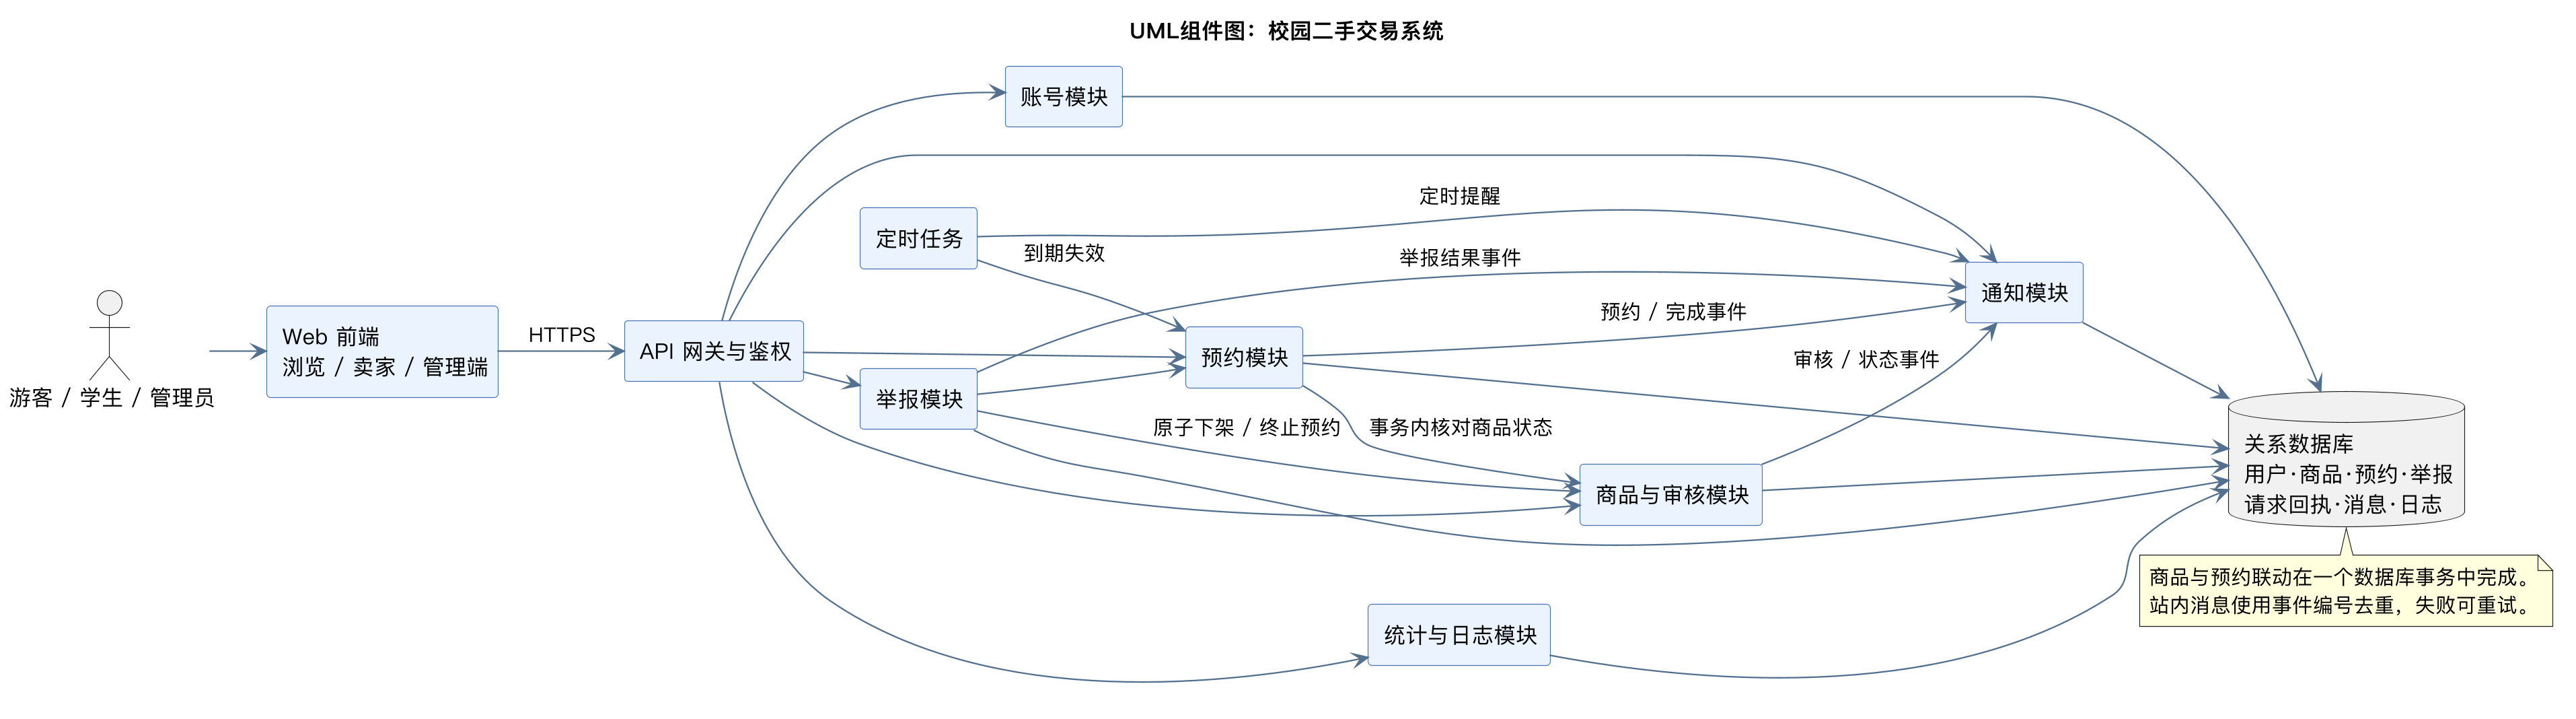
\includegraphics[width=0.9\linewidth,height=\textheight,keepaspectratio,alt={UML组件图（结构性图）：模块间的调用和共享数据库}]{UML/UML组件图.png}
\caption{UML组件图（结构性图）：模块间的调用和共享数据库}
\end{figure}

组件图展示前端、鉴权、商品、预约、举报、通知、统计日志和定时任务的关系。预约模块和举报模块都要读取商品的当前状态；通知模块只在业务提交后接收事件，失败重试不回滚已完成的业务变更。对应
REQ-002、008、015、018、020、023。

\subsection{2.2
领域对象与数据关系}\label{ux9886ux57dfux5bf9ux8c61ux4e0eux6570ux636eux5173ux7cfb}

\begin{figure}
\centering
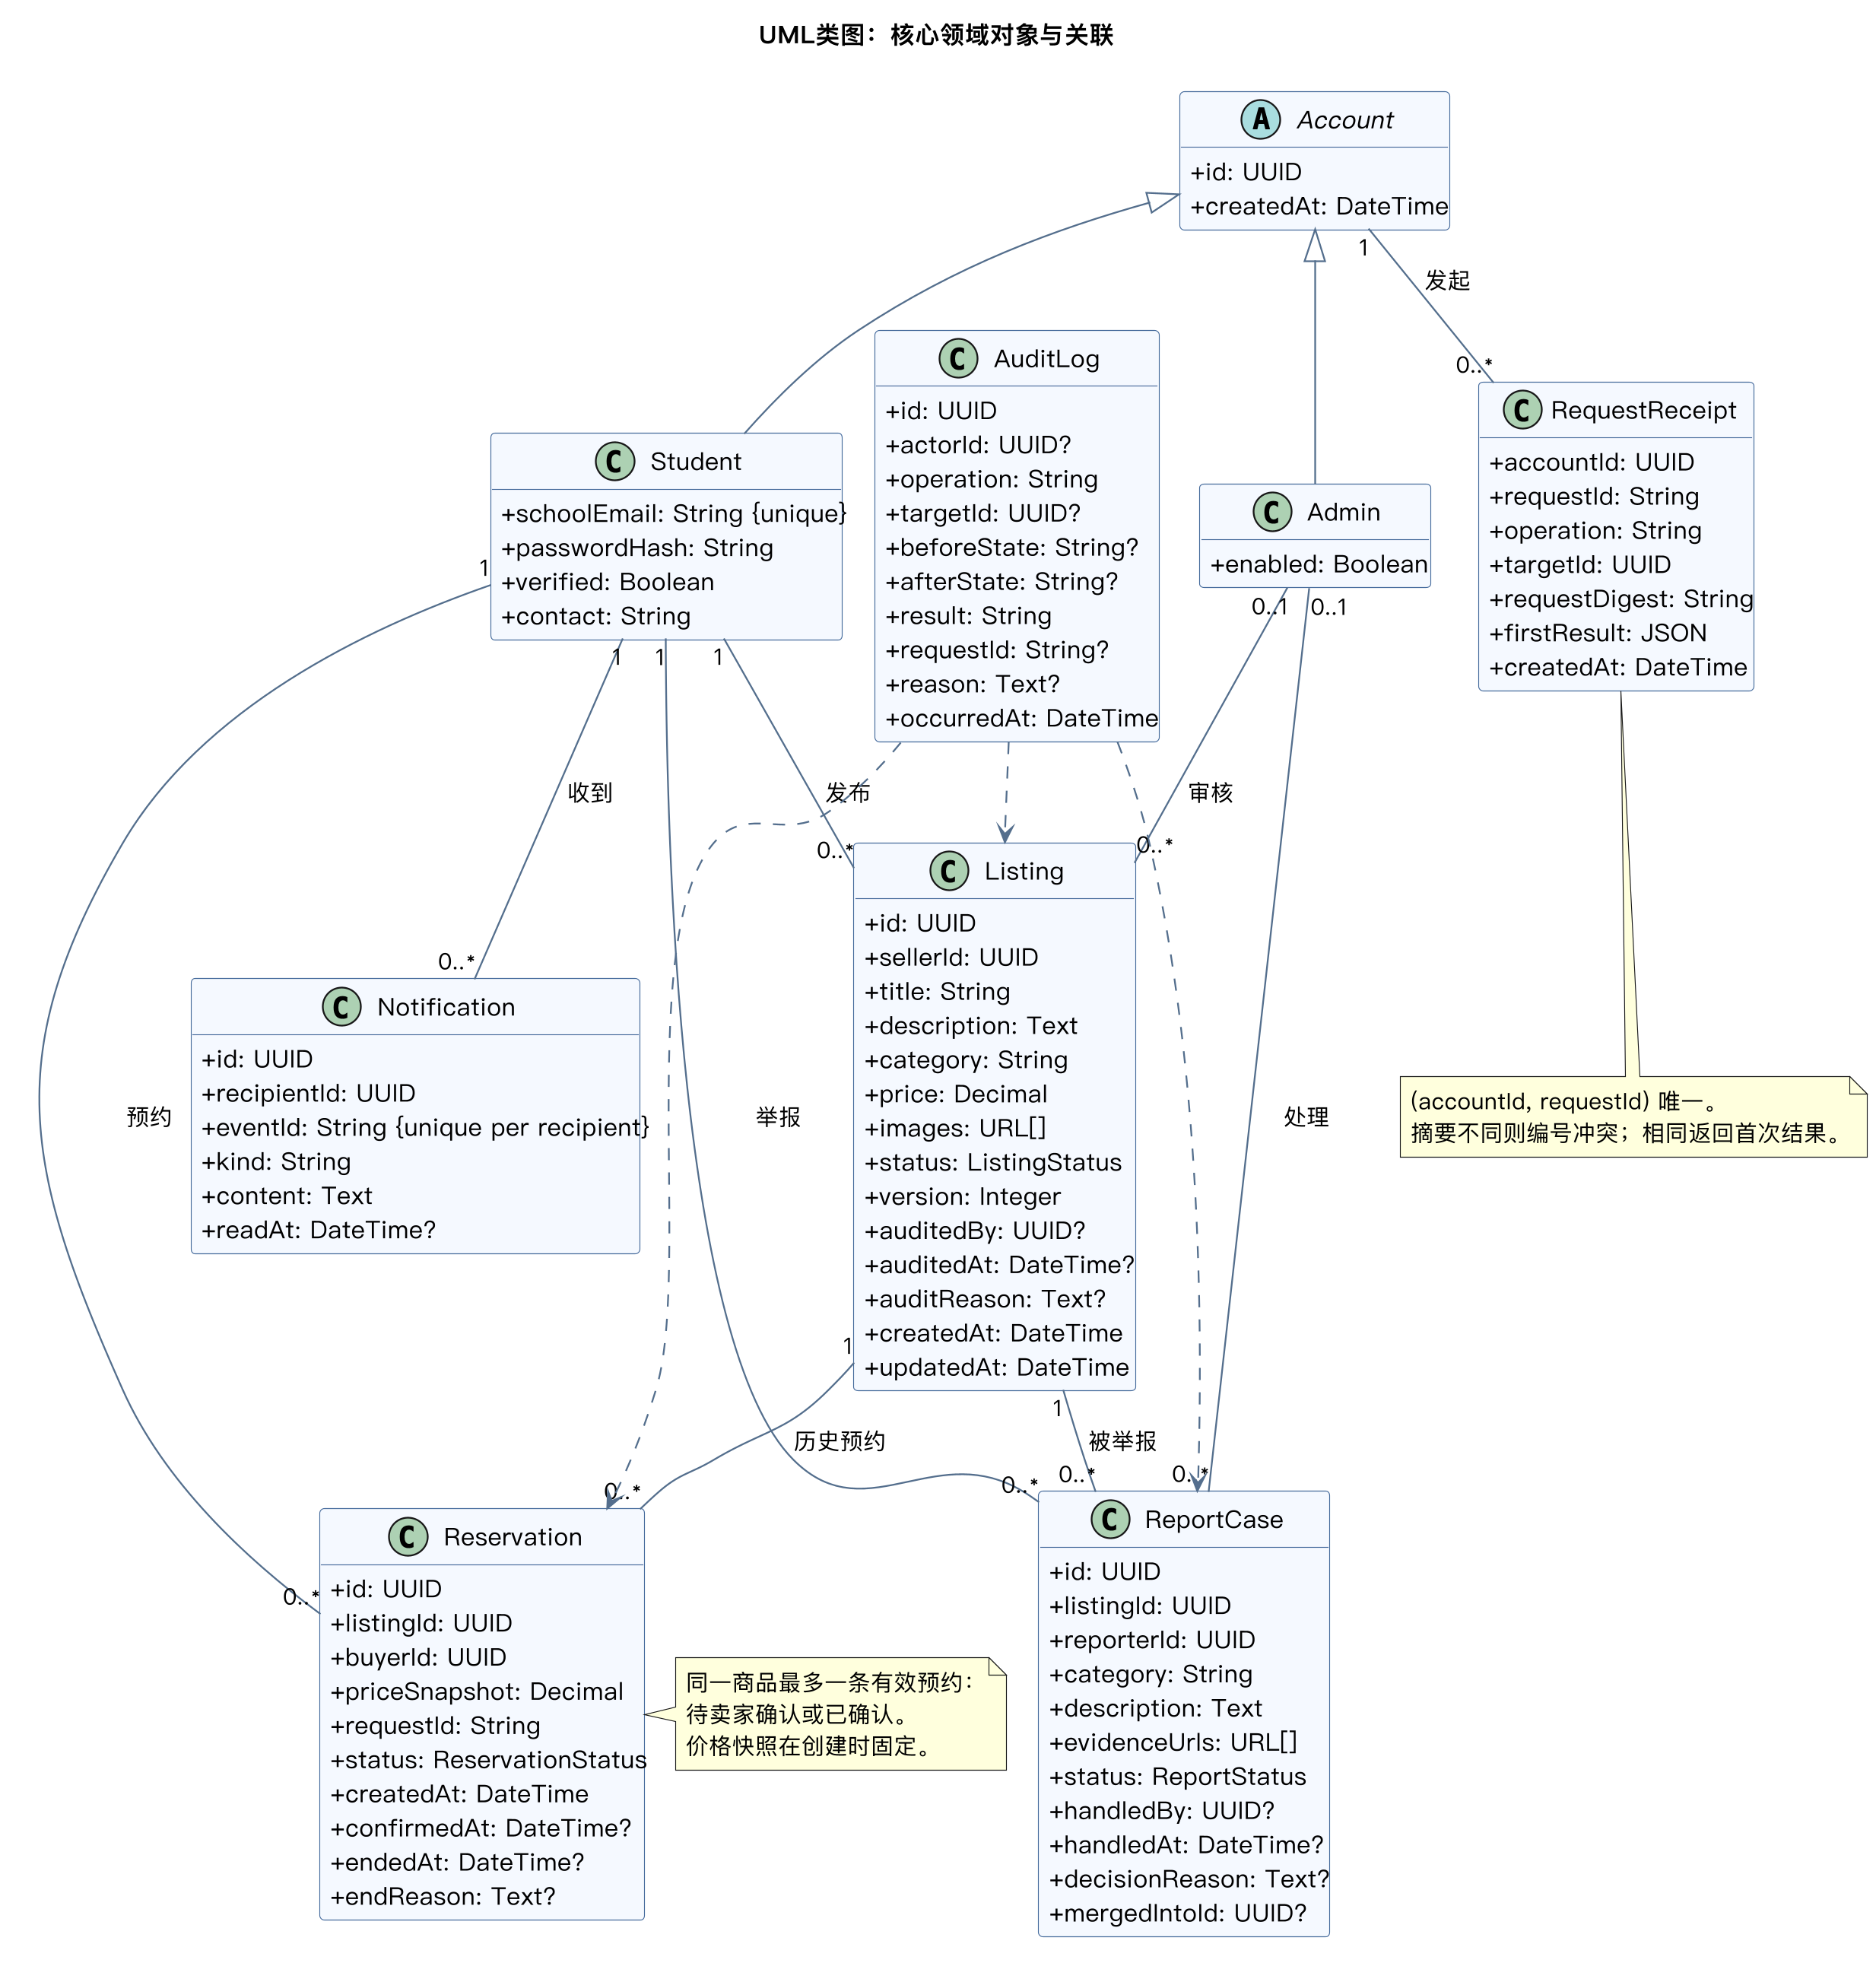
\includegraphics[width=0.95\linewidth,height=\textheight,keepaspectratio,alt={UML类图（必画的结构性图）：核心领域对象与关联}]{UML/UML类图.png}
\caption{UML类图（必画的结构性图）：核心领域对象与关联}
\end{figure}

学生和管理员共享账号编号，但权限不同。商品关联卖家；预约关联买家与商品，并记录创建时的价格快照；举报关联举报人、商品和处理管理员。请求回执记录请求摘要与首次结果，解决重复提交；操作日志记录前后状态与结果，供审计。类图表达数据关系，不能单靠图中的多重性保证``最多一条有效预约''，因此还要在数据库和事务边界落实约束。对应
REQ-001、008、009、015、016、018、020。

{\def\LTcaptype{none} % do not increment counter
\begin{longtable}[]{@{}
  >{\raggedright\arraybackslash}p{(\linewidth - 4\tabcolsep) * \real{0.3333}}
  >{\raggedright\arraybackslash}p{(\linewidth - 4\tabcolsep) * \real{0.3333}}
  >{\raggedright\arraybackslash}p{(\linewidth - 4\tabcolsep) * \real{0.3333}}@{}}
\toprule\noalign{}
\begin{minipage}[b]{\linewidth}\raggedright
核心实体
\end{minipage} & \begin{minipage}[b]{\linewidth}\raggedright
最重要的字段与约束
\end{minipage} & \begin{minipage}[b]{\linewidth}\raggedright
设计原因
\end{minipage} \\
\midrule\noalign{}
\endhead
\bottomrule\noalign{}
\endlastfoot
学生账号 & 学校邮箱唯一、验证状态、密码哈希、联系方式 &
身份验证与联系方式都属于非公开数据。 \\
商品 & 卖家编号、价格、图片、状态、版本、审核信息 &
版本用于识别旧页面提交；发布后修改必须重审。 \\
预约 & 买家、商品、价格快照、状态、创建/确认/结束时间与原因 &
交易统计按历史成交价，不按后来商品价格。 \\
请求回执 & 账号、请求编号、操作、目标、参数摘要、首次结果 &
同账号同编号相同内容返回首次结果，内容不同报冲突。 \\
举报 & 举报人、商品、状态、理由、处理人及合并关联 &
一件商品有多条举报时可追踪合并与失效关闭。 \\
通知与日志 & 事件编号/收件人；操作人/目标/前后状态/结果 &
消息去重；关键操作追加记录。 \\
\end{longtable}
}

\subsection{2.3
参与者与功能边界}\label{ux53c2ux4e0eux8005ux4e0eux529fux80fdux8fb9ux754c}

\begin{figure}
\centering
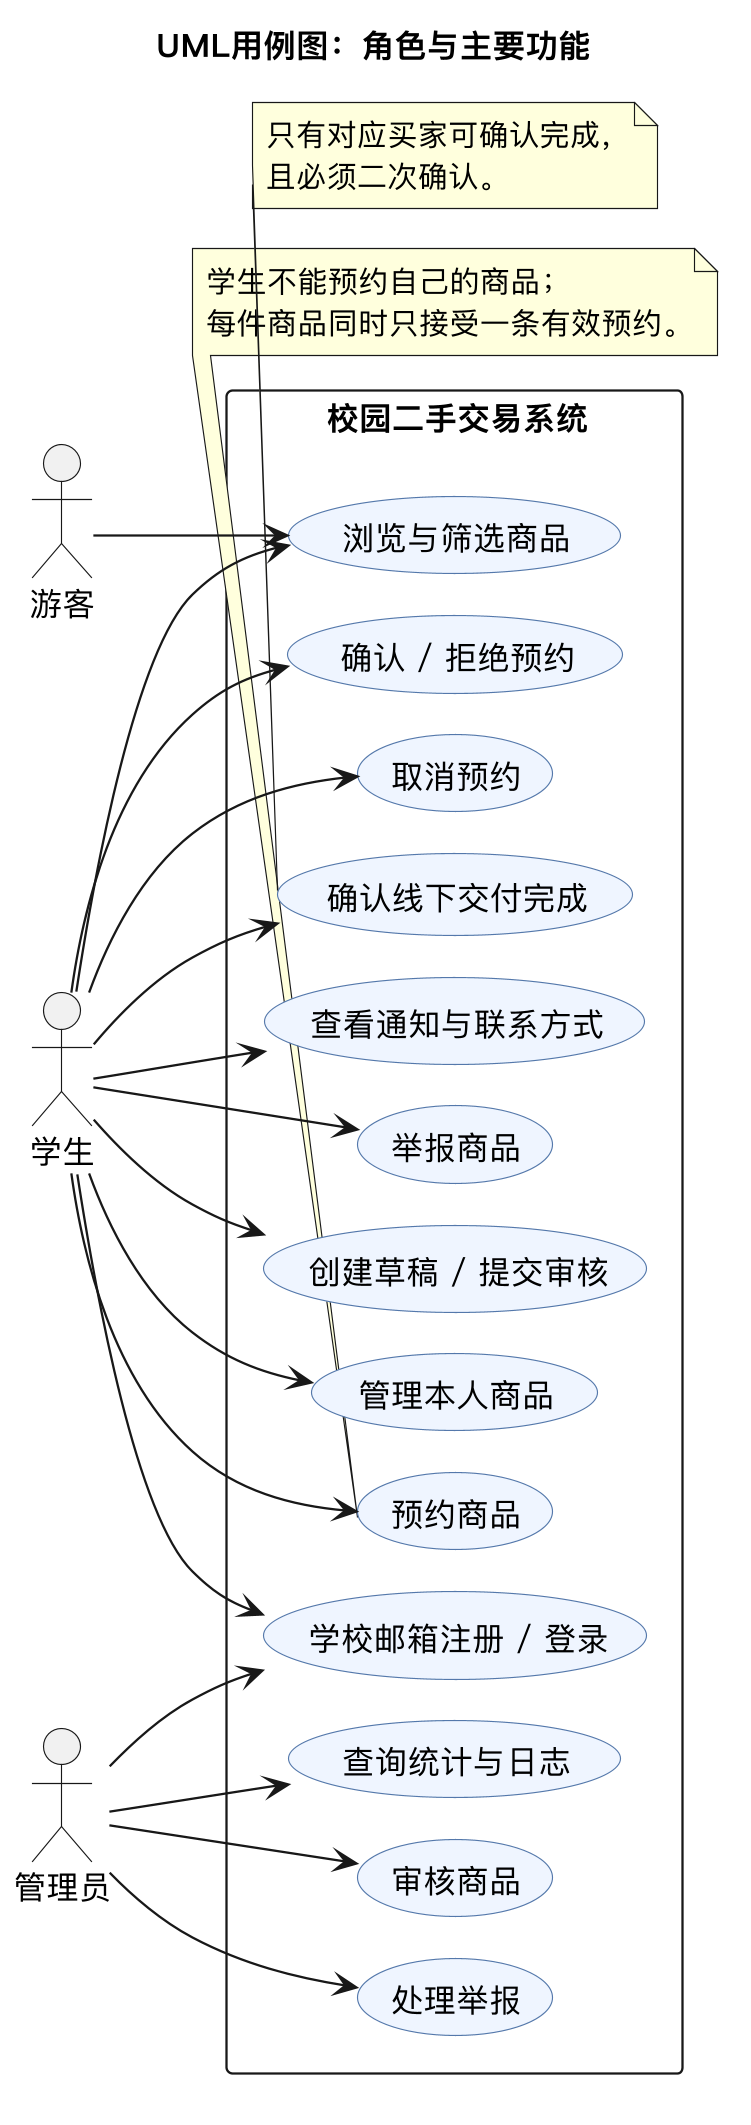
\includegraphics[width=\linewidth,height=20cm,keepaspectratio,alt={UML用例图（行为性图）：游客、学生和管理员的功能边界}]{UML/UML用例图.png}
\caption{UML用例图（行为性图）：游客、学生和管理员的功能边界}
\end{figure}

同一个学生账号既能买也能卖，因此用例图用``学生''作为统一参与者，没有另设需要切换的买家、卖家账号。管理员只有审核、举报、统计和日志权限，不能代替买家确认线下交付；游客只能浏览公开商品。对应
REQ-001、002、026。

\subsection{2.4 状态规则}\label{ux72b6ux6001ux89c4ux5219}

\begin{figure}
\centering
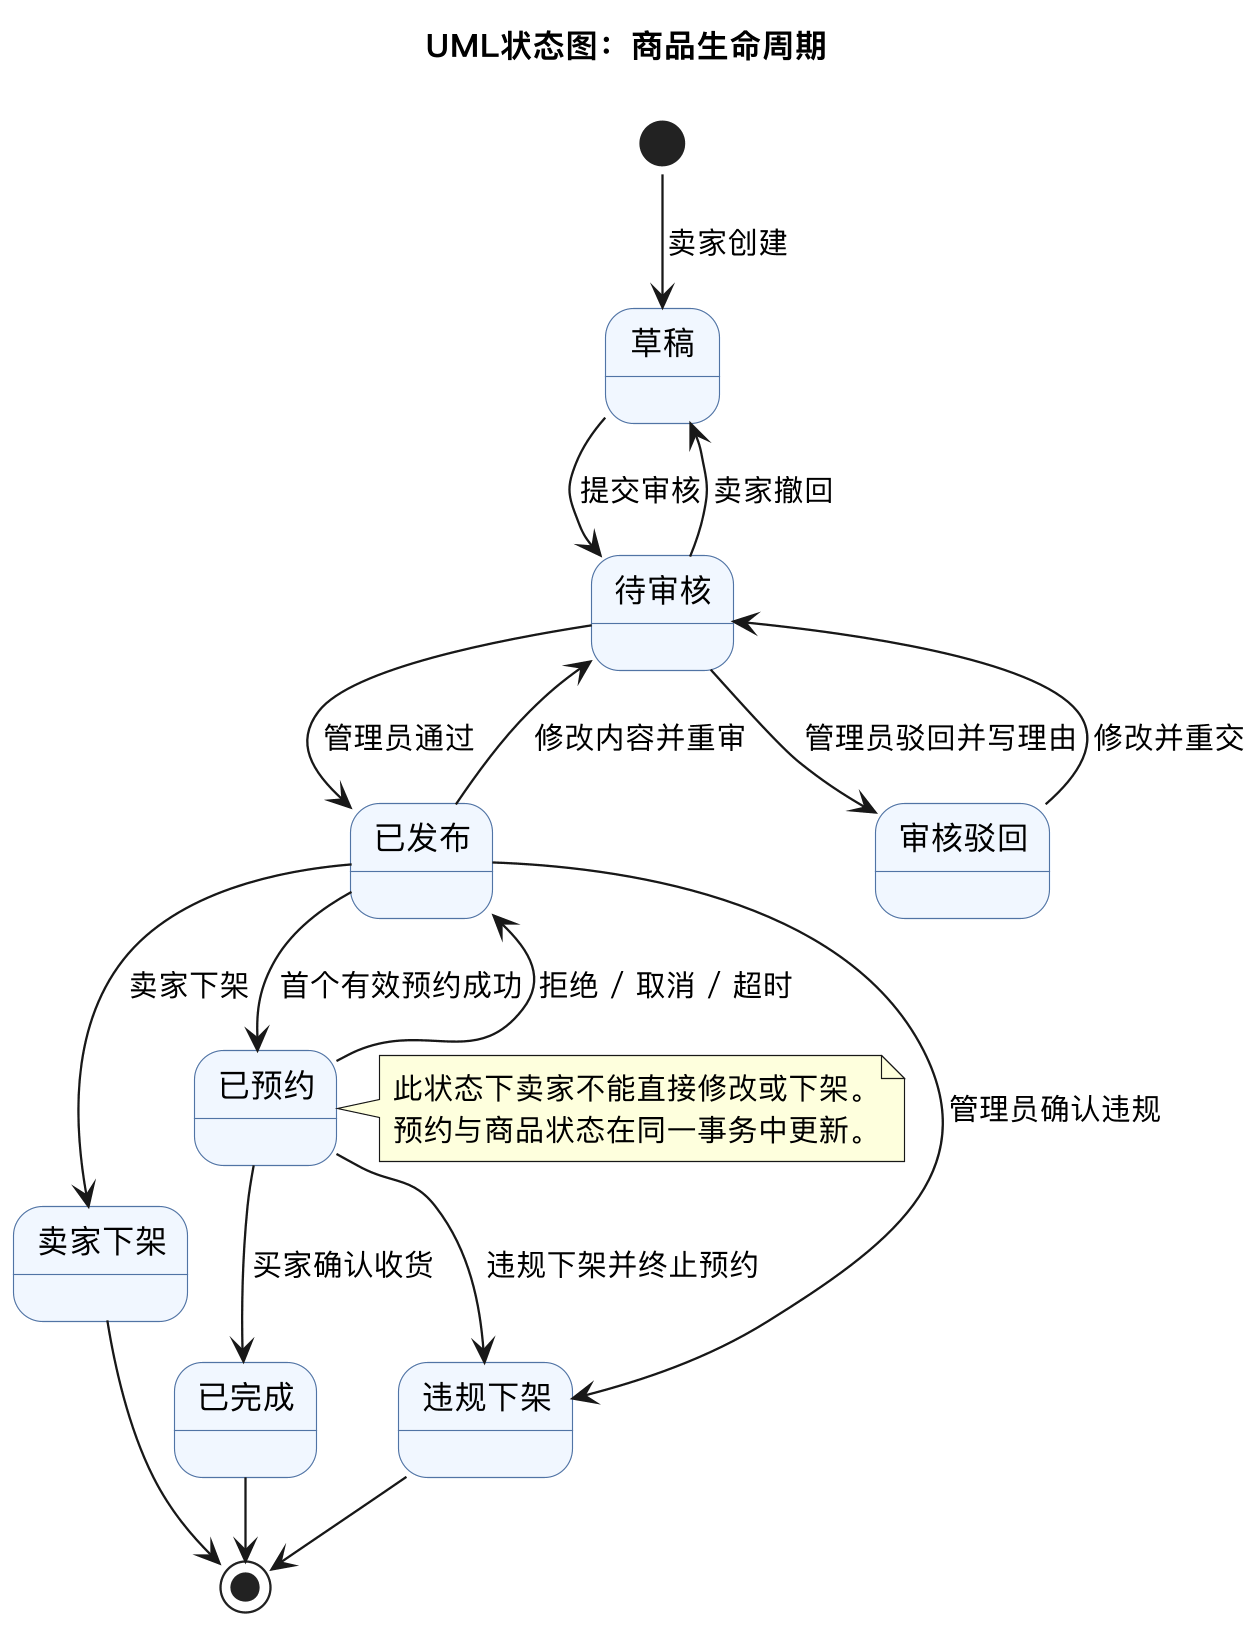
\includegraphics[width=0.86\linewidth,height=\textheight,keepaspectratio,alt={UML商品状态图（行为性图）：草稿、审核、发布、预约和终态}]{UML/UML商品状态图.png}
\caption{UML商品状态图（行为性图）：草稿、审核、发布、预约和终态}
\end{figure}

商品已预约时不能直接改内容或下架；预约正常解除才恢复已发布。已完成、卖家下架、违规下架均为终态。待审核商品不公开展示。对应
REQ-003---005、008、014、015。

\begin{figure}
\centering
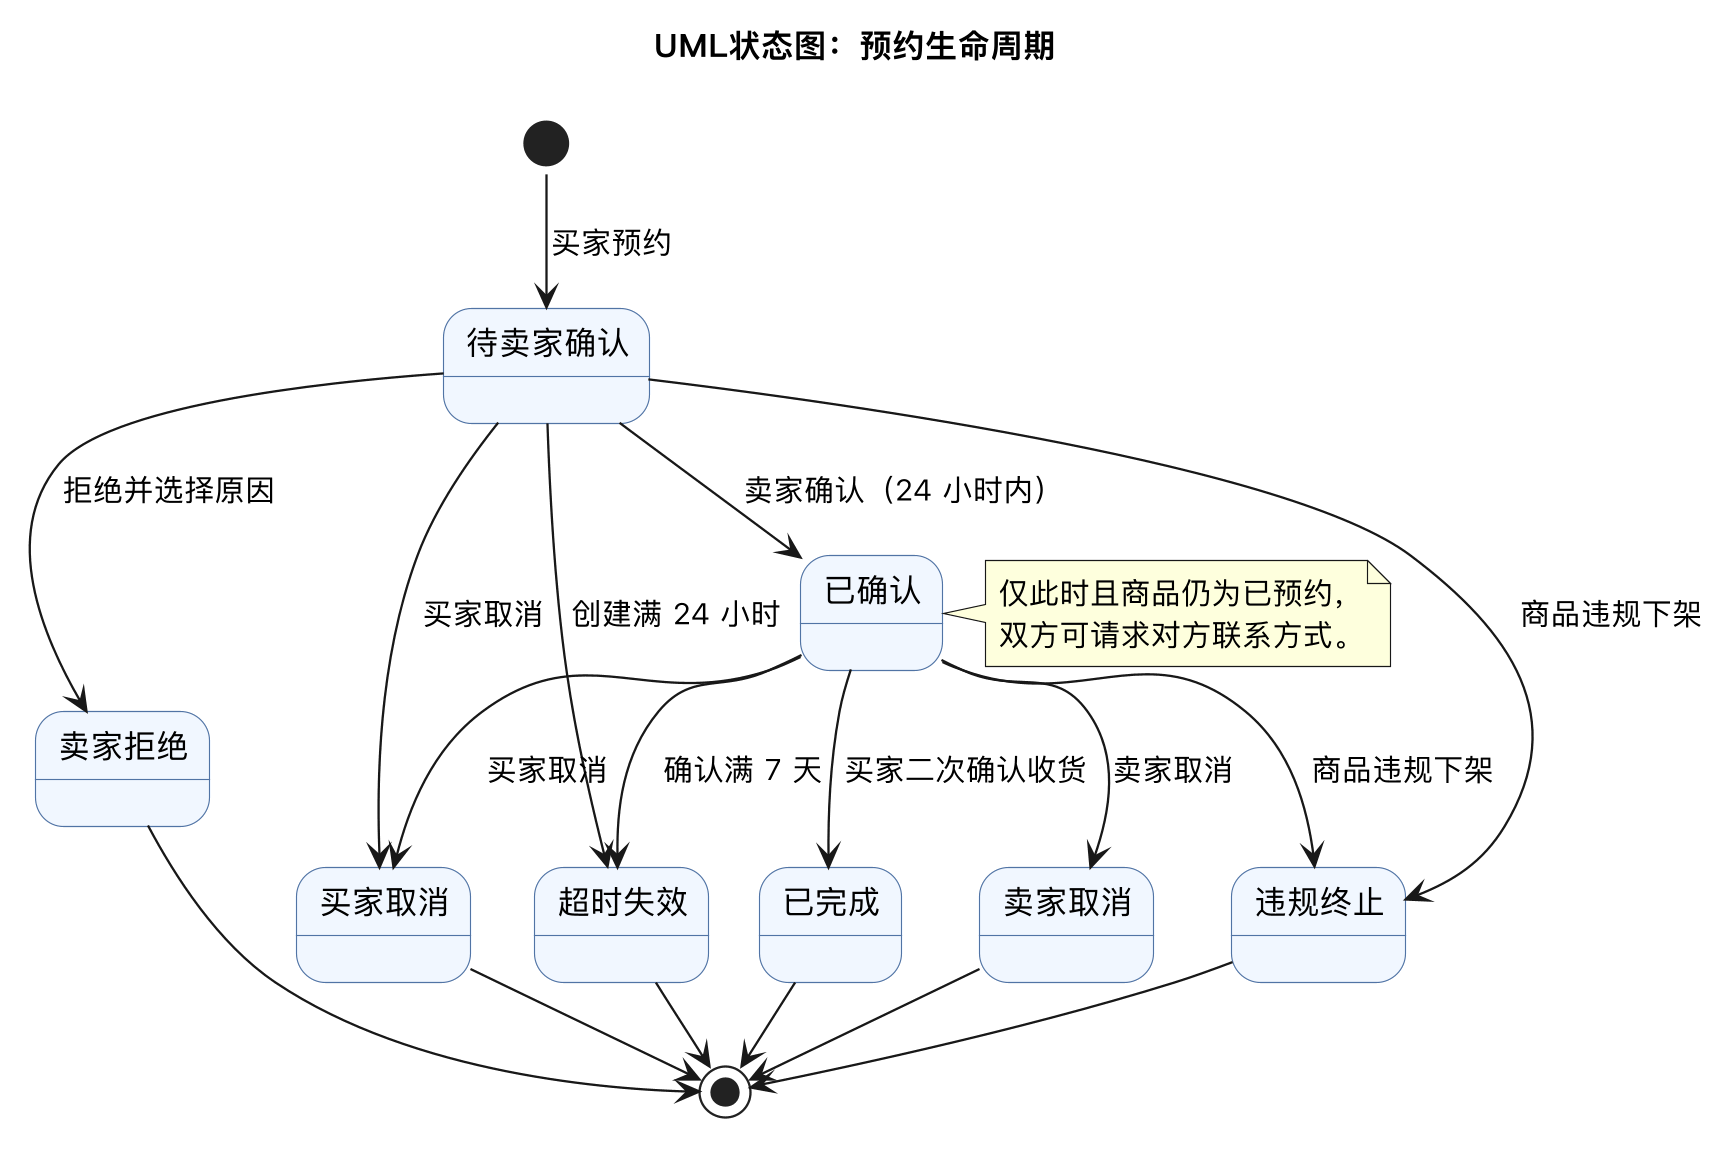
\includegraphics[width=0.88\linewidth,height=\textheight,keepaspectratio,alt={UML预约状态图（行为性图）：待确认、已确认与结束原因}]{UML/UML预约状态图.png}
\caption{UML预约状态图（行为性图）：待确认、已确认与结束原因}
\end{figure}

只有``待卖家确认''和``已确认''是有效预约。待确认从创建起 24
小时到期；已确认从确认起 7
天到期，超时只表示预约结束，不表示交易完成。联系方式读取还须同时满足商品仍``已预约''；预约结束后服务端立即停止提供对方联系方式。对应
REQ-011---014、019、024。

\subsection{2.5 关键交互}\label{ux5173ux952eux4ea4ux4e92}

\begin{figure}
\centering
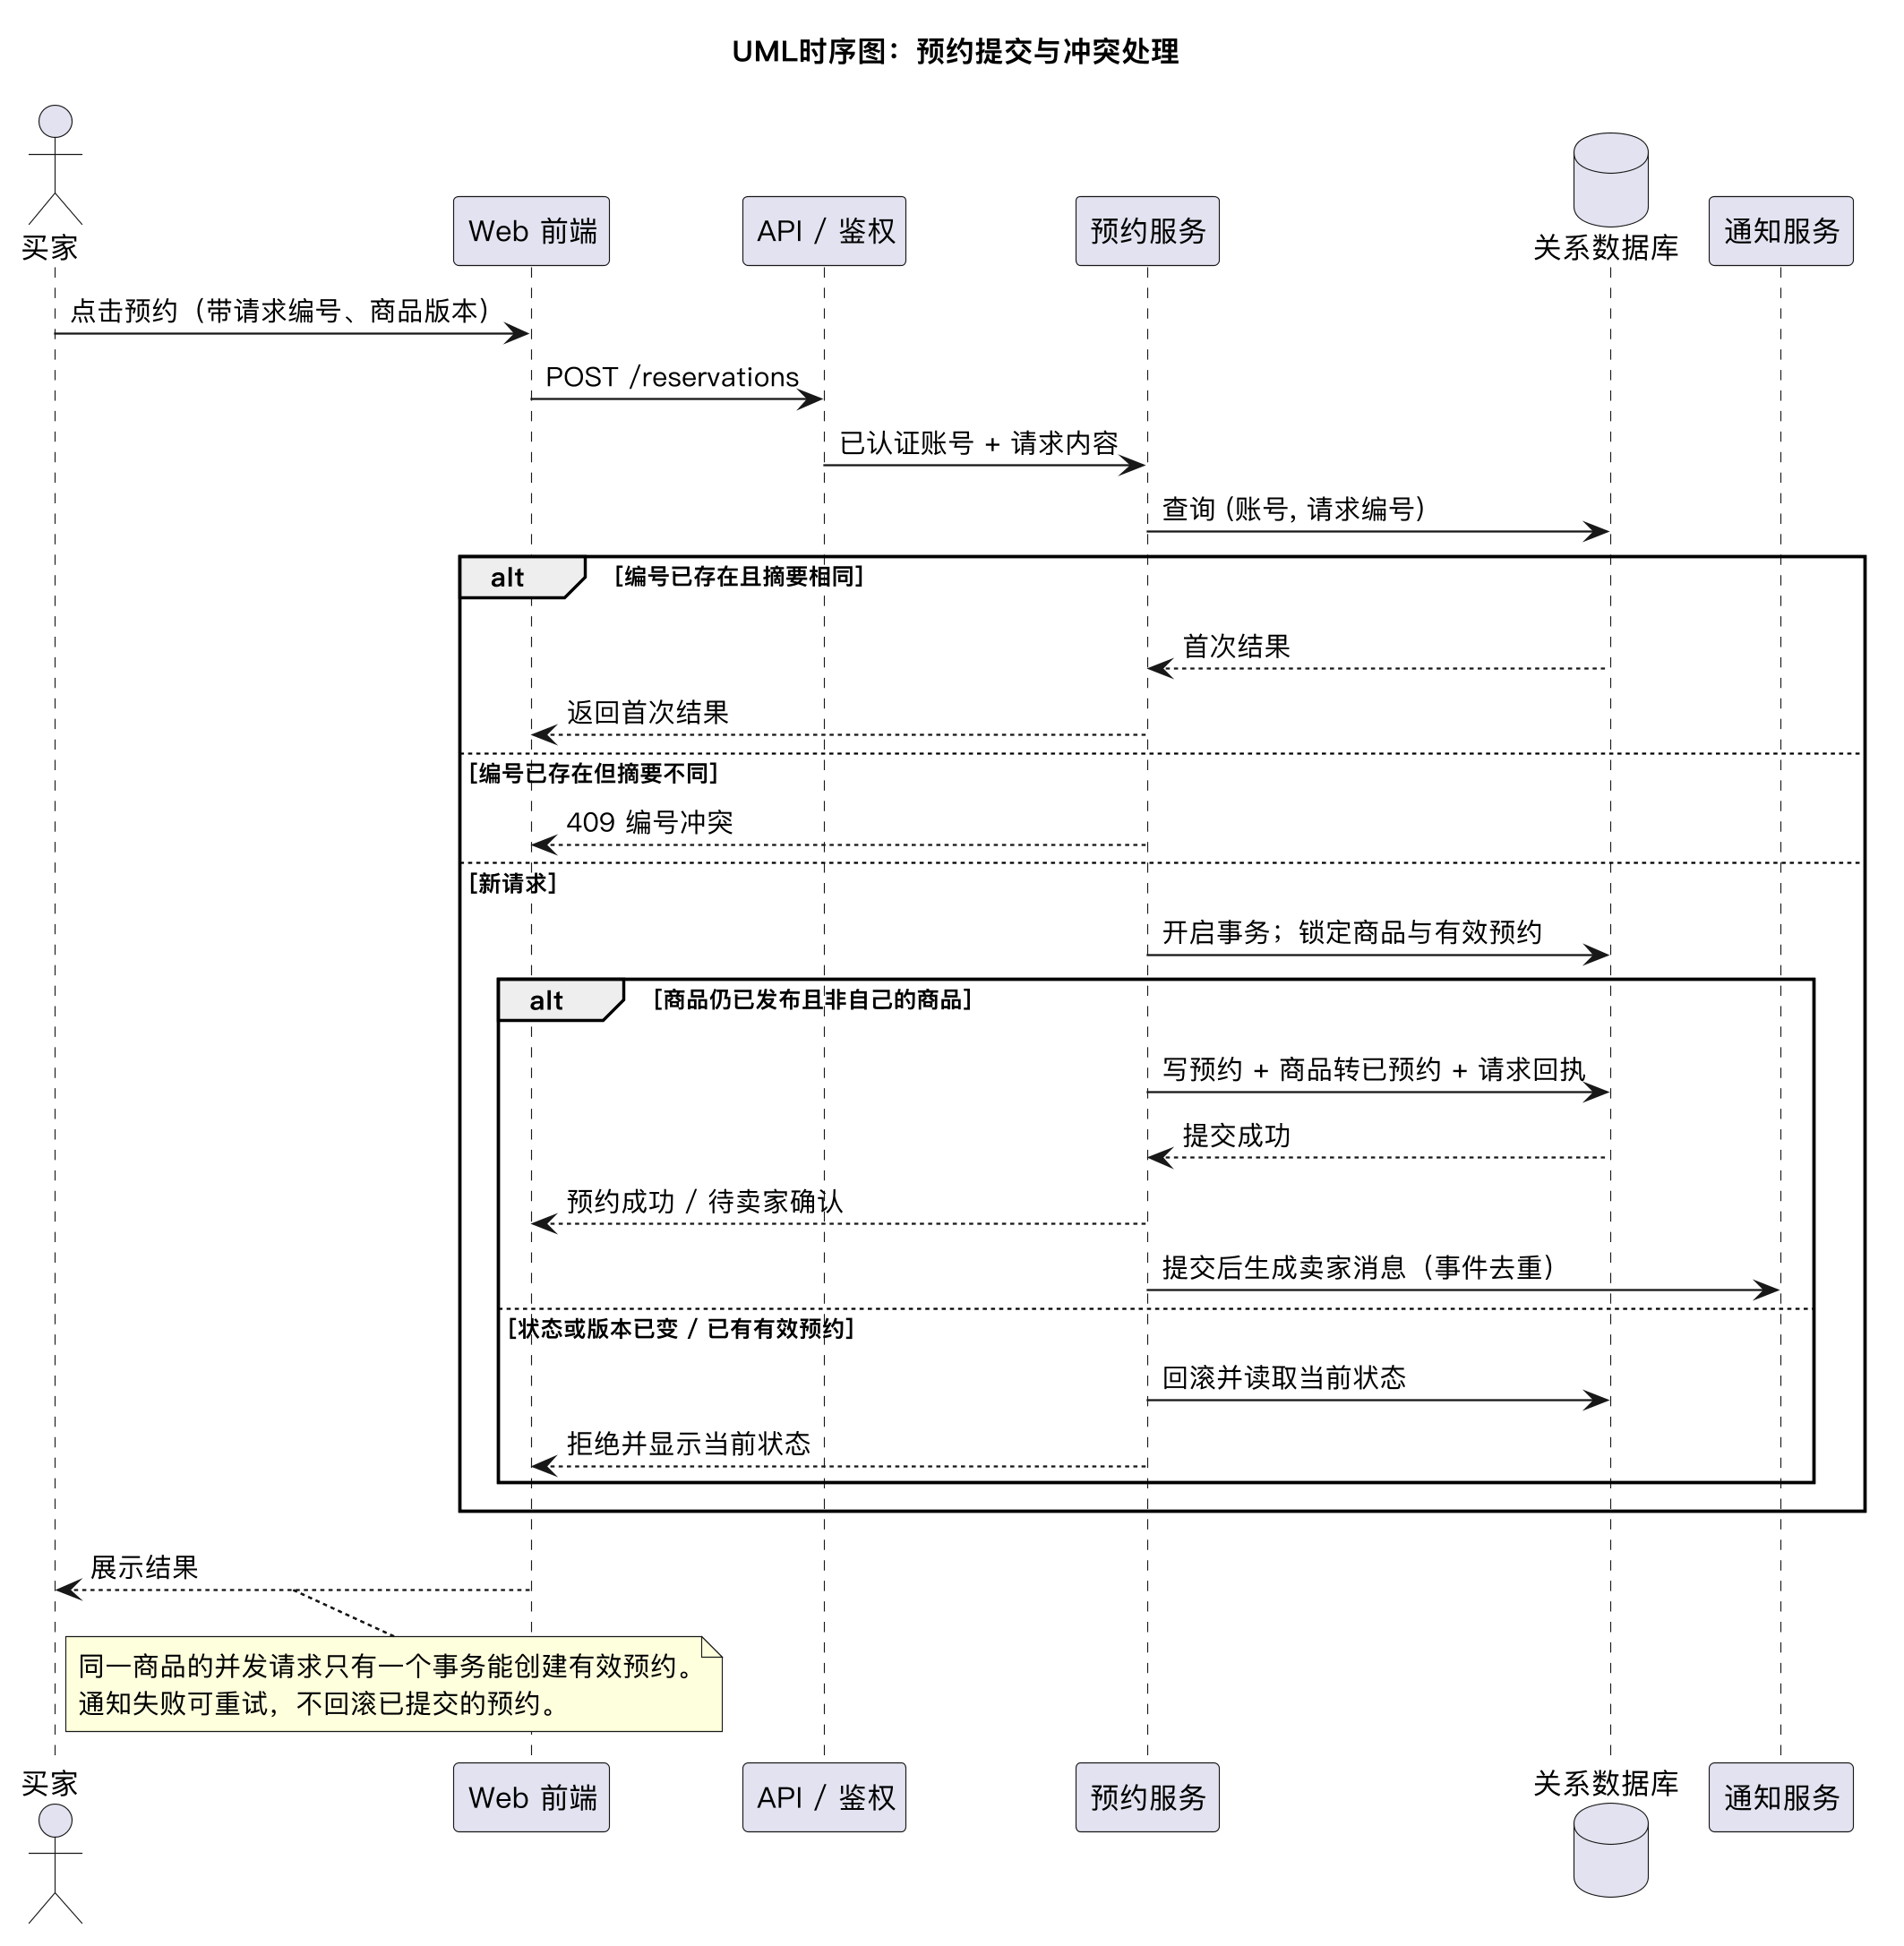
\includegraphics[width=\linewidth,height=16cm,keepaspectratio,alt={UML预约时序图（交互性图）：幂等、编号冲突与并发预约}]{UML/UML预约时序图.png}
\caption{UML预约时序图（交互性图）：幂等、编号冲突与并发预约}
\end{figure}

时序图要求前端提交请求编号和页面看到的商品版本。服务端先查请求回执：内容完全相同则返回首次结果，编号相同但内容不同则拒绝。新请求进入事务，锁定商品并检查是否已有有效预约；成功时原子写入预约、商品状态和回执，失败时返回最新状态。站内消息在事务成功后生成，并以事件编号去重。对应
REQ-008---010、016、018、023。

\subsection{2.6
跨模块规则检查}\label{ux8de8ux6a21ux5757ux89c4ux5219ux68c0ux67e5}

{\def\LTcaptype{none} % do not increment counter
\begin{longtable}[]{@{}
  >{\raggedright\arraybackslash}p{(\linewidth - 4\tabcolsep) * \real{0.3333}}
  >{\raggedright\arraybackslash}p{(\linewidth - 4\tabcolsep) * \real{0.3333}}
  >{\raggedright\arraybackslash}p{(\linewidth - 4\tabcolsep) * \real{0.3333}}@{}}
\toprule\noalign{}
\begin{minipage}[b]{\linewidth}\raggedright
场景
\end{minipage} & \begin{minipage}[b]{\linewidth}\raggedright
设计处理
\end{minipage} & \begin{minipage}[b]{\linewidth}\raggedright
对应图/界面
\end{minipage} \\
\midrule\noalign{}
\endhead
\bottomrule\noalign{}
\endlastfoot
两人同时预约 & 商品与有效预约在同一事务里检查和更新，仅一人成功。 &
组件图、时序图；界面 03、06 \\
旧页面提交 & 校验版本与状态，不覆盖新值；提示用户刷新。 & 时序图；界面
05、09 \\
同编号不同请求 & \texttt{(账号,\ 请求编号)}
查到不同摘要，拒绝为编号冲突。 & 类图、时序图 \\
商品完成与违规下架竞争 & 处理前原子核对商品现态；先提交者生效。 &
组件图、状态图；界面 10 \\
预约终态后查看联系方式 &
每次请求都校验预约和商品状态，历史页不保存联系方式快照。 &
预约状态图；界面 06 \\
消息任务重试 & 以业务事件编号与收件人去重，不回滚已提交业务。 &
组件图；界面 07 \\
\end{longtable}
}

\section{3 UI 界面设计}\label{ui-ux754cux9762ux8bbeux8ba1}

界面设计先用 ReportLab 确定布局草稿，再到 Figma 中重建为十一张独立的
1440 × 900
画板。正式原型见\href{https://www.figma.com/design/iOritXAT7LrtlUUrjtuZBn}{校园集市
Figma
设计文件}，文字、图形和配色都可以继续编辑；下文图片均为对应画板导出的
PNG。各页统一采用左侧导航、顶部标题、卡片内容和明确的状态标签，用于检查信息层次与操作路径。界面是设计原型，并非已经运行的前端。

{\def\LTcaptype{none} % do not increment counter
\begin{longtable}[]{@{}
  >{\raggedright\arraybackslash}p{(\linewidth - 4\tabcolsep) * \real{0.3333}}
  >{\raggedright\arraybackslash}p{(\linewidth - 4\tabcolsep) * \real{0.3333}}
  >{\raggedright\arraybackslash}p{(\linewidth - 4\tabcolsep) * \real{0.3333}}@{}}
\toprule\noalign{}
\begin{minipage}[b]{\linewidth}\raggedright
界面
\end{minipage} & \begin{minipage}[b]{\linewidth}\raggedright
所在模块 / 主要功能
\end{minipage} & \begin{minipage}[b]{\linewidth}\raggedright
关键规则
\end{minipage} \\
\midrule\noalign{}
\endhead
\bottomrule\noalign{}
\endlastfoot
01 注册登录 & 账号；邮箱验证、设置密码 & 学校域名留作配置项。 \\
02 商品浏览 & 商品查询；关键词、分类、价格筛选与排序 &
仅展示已发布可预约商品。 \\
03 商品详情与预约 & 商品、预约；查看详情、预约、举报入口 &
确认前不显示联系方式。 \\
04 卖家商品管理 & 商品；草稿、审核、发布、下架列表 &
已发布修改要重审，已预约不可直接下架。 \\
05 卖家处理预约 & 预约；确认或拒绝 & 24 小时内操作，拒绝需选原因。 \\
06 买家预约详情 & 预约；线下联系、二次确认完成 &
联系方式按现态提供；完成不可撤销。 \\
07 站内消息 & 通知；业务消息与定时提醒 & 12
小时进度提醒、确认期到期前提醒。 \\
08 提交举报 & 举报；类别、说明、可选图片 & 重复待处理举报返回原记录。 \\
09 管理员商品审核 & 商品审核；通过或驳回 &
驳回填写理由，旧页面提交前重新读现态。 \\
10 管理员举报处理 & 举报处理；驳回或违规下架 &
并发核对、合并同商品举报。 \\
11 统计与日志 & 统计、日志；成交额、操作查询 &
只计已完成预约；全局日志仅管理员可看。 \\
\end{longtable}
}

\subsection{3.1 学生端界面}\label{ux5b66ux751fux7aefux754cux9762}

\subsubsection{界面 01
注册登录}\label{ux754cux9762-01-ux6ce8ux518cux767bux5f55}

\begin{figure}
\centering
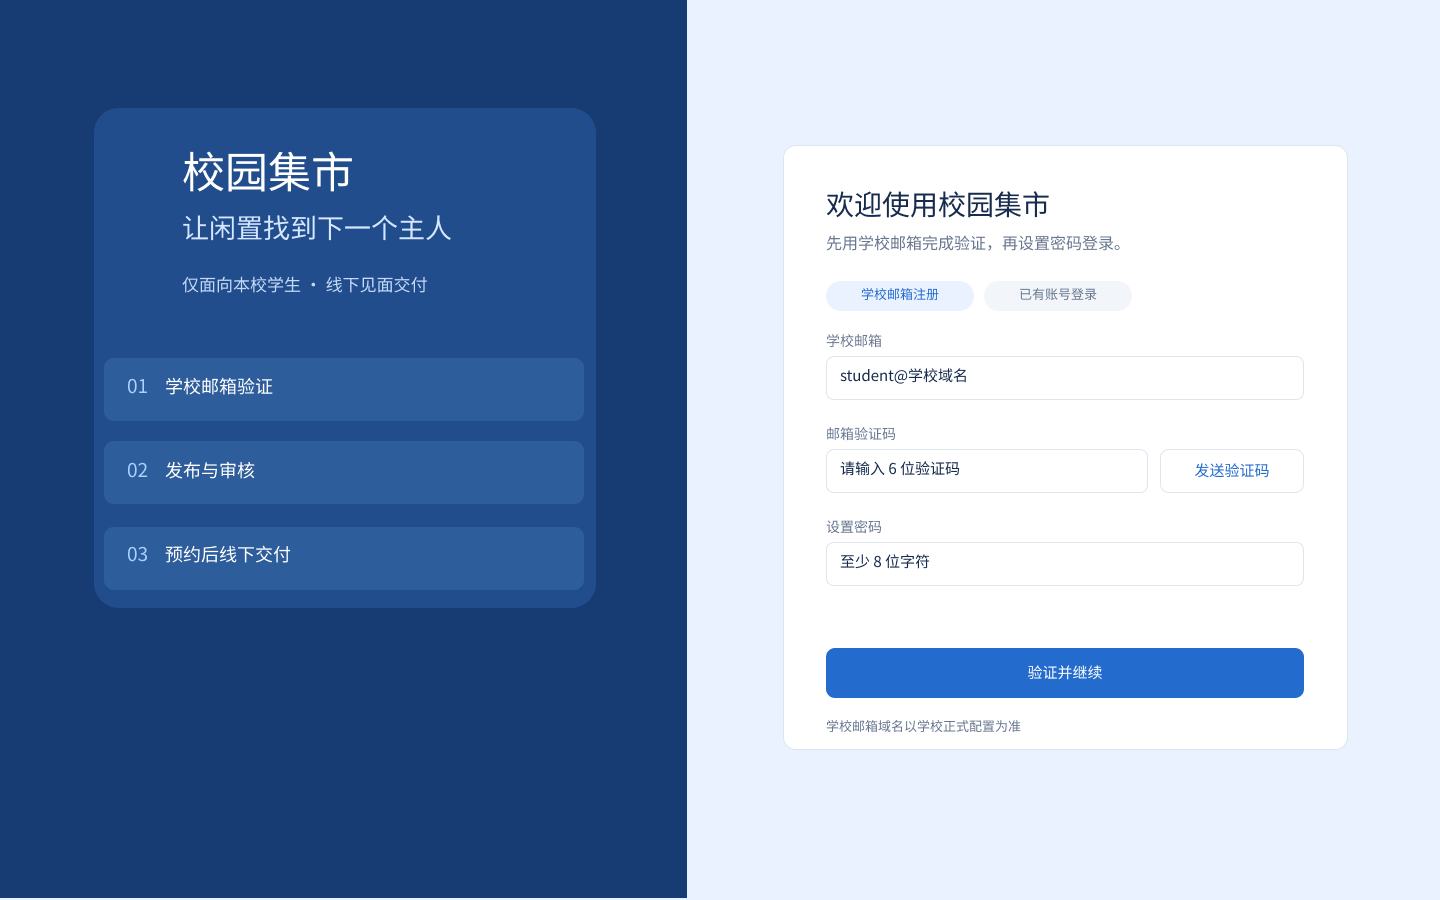
\includegraphics[width=0.88\linewidth,height=\textheight,keepaspectratio,alt={注册登录}]{UI界面/01_注册登录.png}
\caption{注册登录}
\end{figure}

输入学校邮箱并获取验证码，验证后设置密码。真实学校域名尚未确认，原型使用说明文字而不伪造具体域名。

\subsubsection{界面 02
商品浏览}\label{ux754cux9762-02-ux5546ux54c1ux6d4fux89c8}

\begin{figure}
\centering
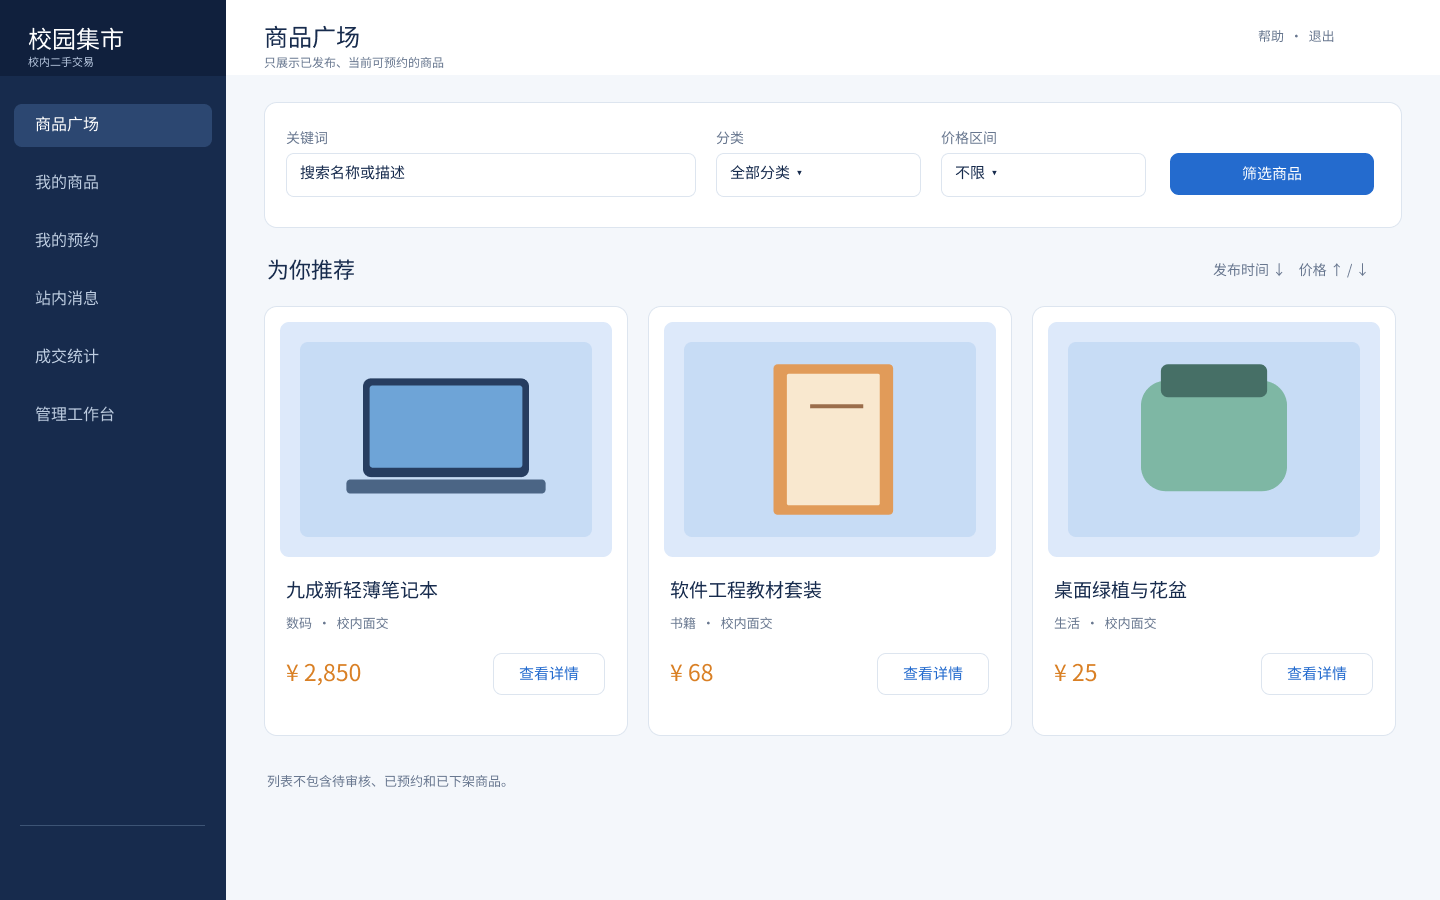
\includegraphics[width=0.88\linewidth,height=\textheight,keepaspectratio,alt={商品浏览}]{UI界面/02_商品浏览.png}
\caption{商品浏览}
\end{figure}

列表组合筛选关键词、分类和价格区间；默认按发布时间倒序。状态已预约、待审核或下架的商品不在公开列表。

\subsubsection{界面 03
商品详情与预约}\label{ux754cux9762-03-ux5546ux54c1ux8be6ux60c5ux4e0eux9884ux7ea6}

\begin{figure}
\centering
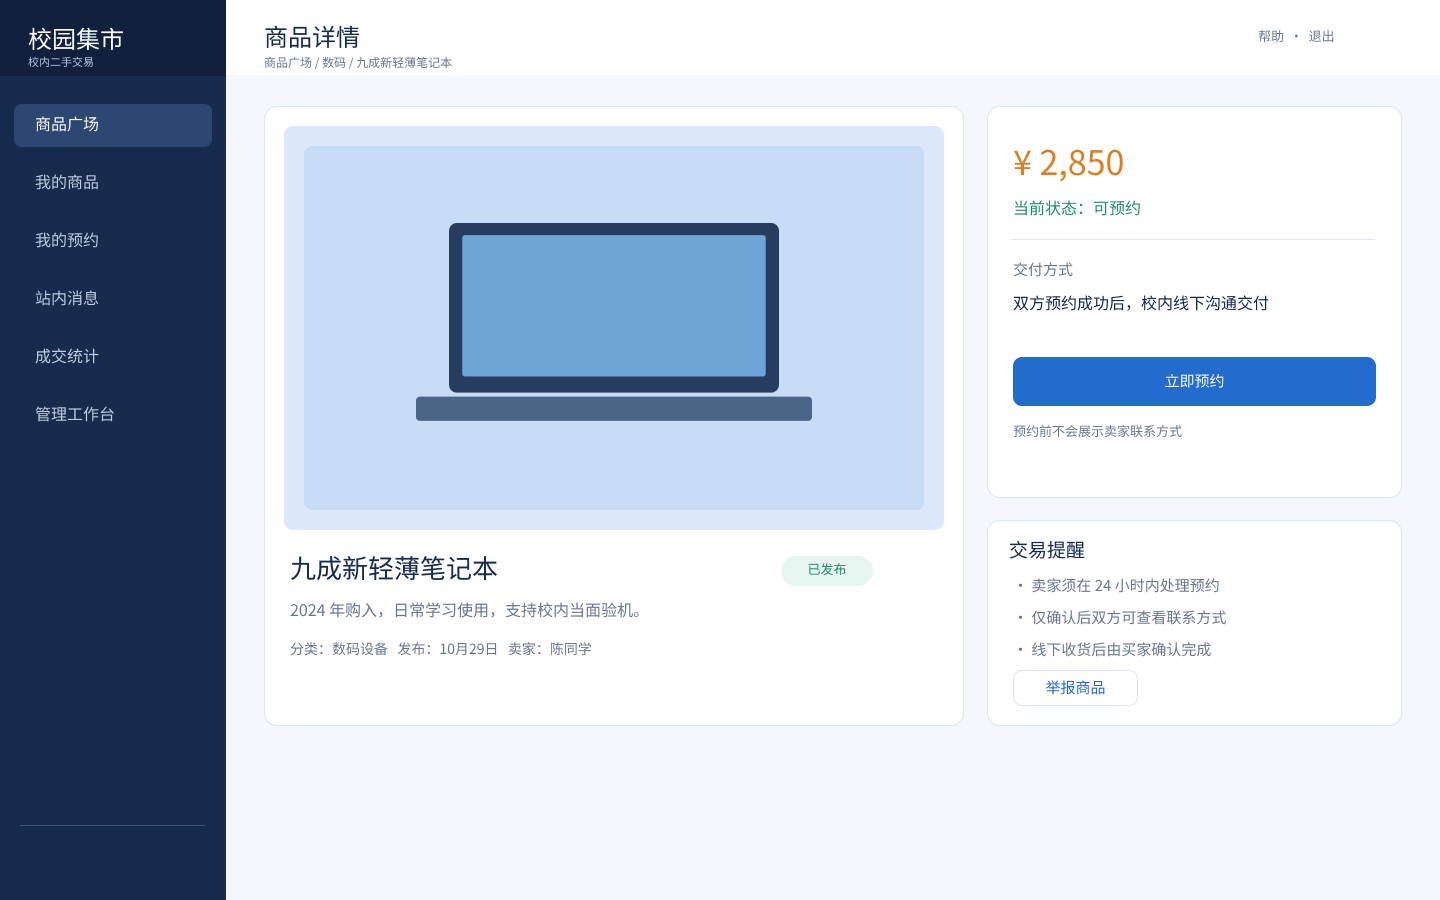
\includegraphics[width=0.88\linewidth,height=\textheight,keepaspectratio,alt={商品详情与预约}]{UI界面/03_商品详情与预约.png}
\caption{商品详情与预约}
\end{figure}

商品详情展示价格、卖家、校内交付说明以及预约按钮。举报作为独立入口；预约前不能读取卖家的联系方式。

\subsubsection{界面 04
卖家商品管理}\label{ux754cux9762-04-ux5356ux5bb6ux5546ux54c1ux7ba1ux7406}

\begin{figure}
\centering
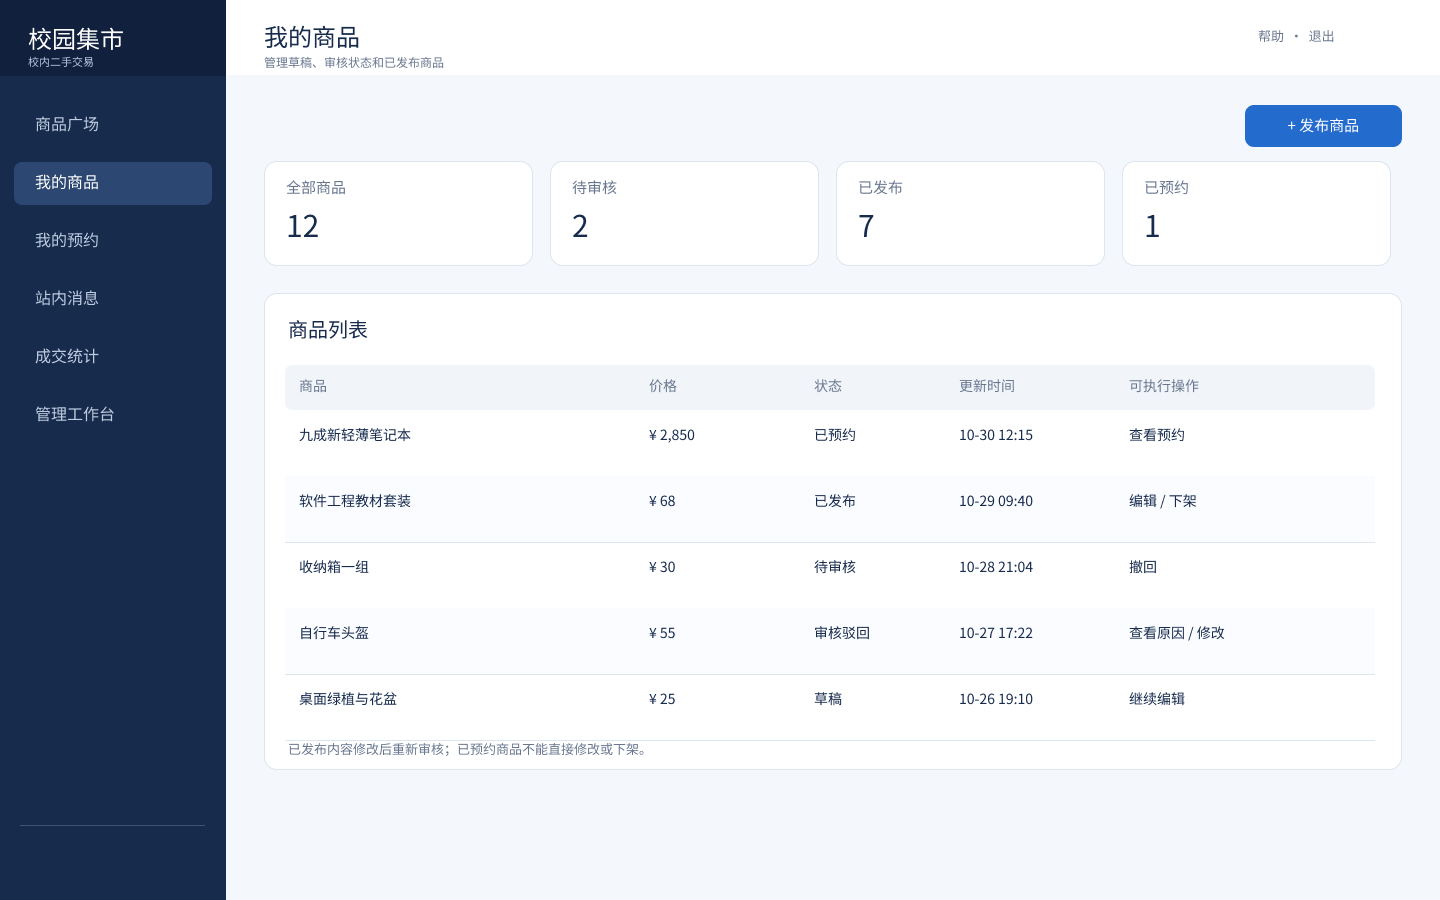
\includegraphics[width=0.88\linewidth,height=\textheight,keepaspectratio,alt={卖家商品管理}]{UI界面/04_卖家商品管理.png}
\caption{卖家商品管理}
\end{figure}

卖家按状态查本人商品；不同状态只显示可执行操作。已发布商品编辑后回到审核，已预约商品不能直接下架。

\subsubsection{界面 05
卖家处理预约}\label{ux754cux9762-05-ux5356ux5bb6ux5904ux7406ux9884ux7ea6}

\begin{figure}
\centering
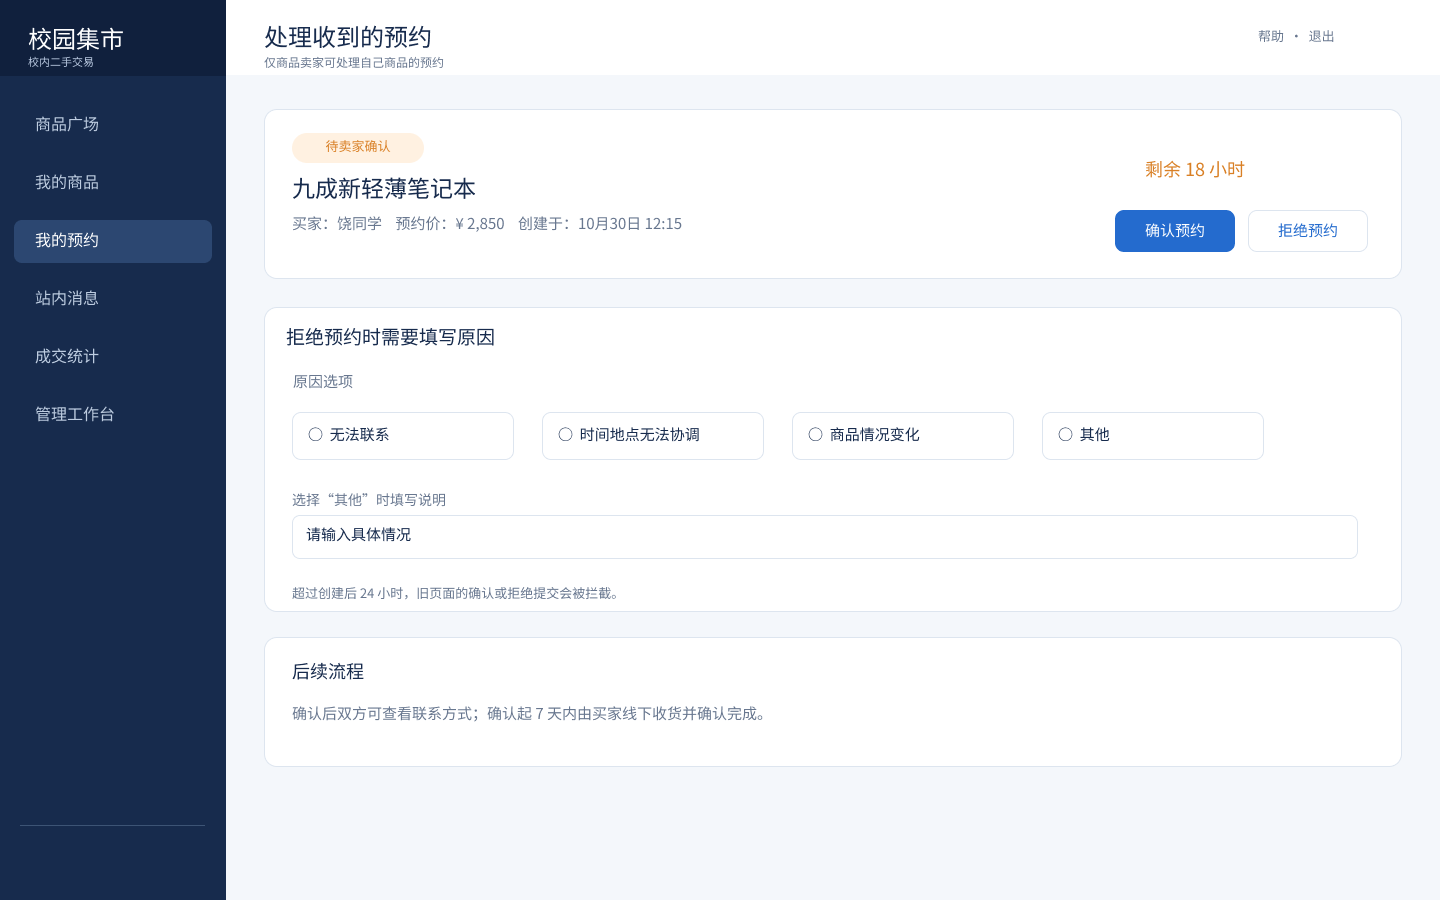
\includegraphics[width=0.88\linewidth,height=\textheight,keepaspectratio,alt={卖家处理预约}]{UI界面/05_卖家处理预约.png}
\caption{卖家处理预约}
\end{figure}

显示预约创建时间、剩余处理时长及确认/拒绝操作。拒绝原因采用固定选项；选``其他''需补充说明。实际提交时服务端再次检查
24 小时期和预约状态。

\subsubsection{界面 06
买家预约详情}\label{ux754cux9762-06-ux4e70ux5bb6ux9884ux7ea6ux8be6ux60c5}

\begin{figure}
\centering
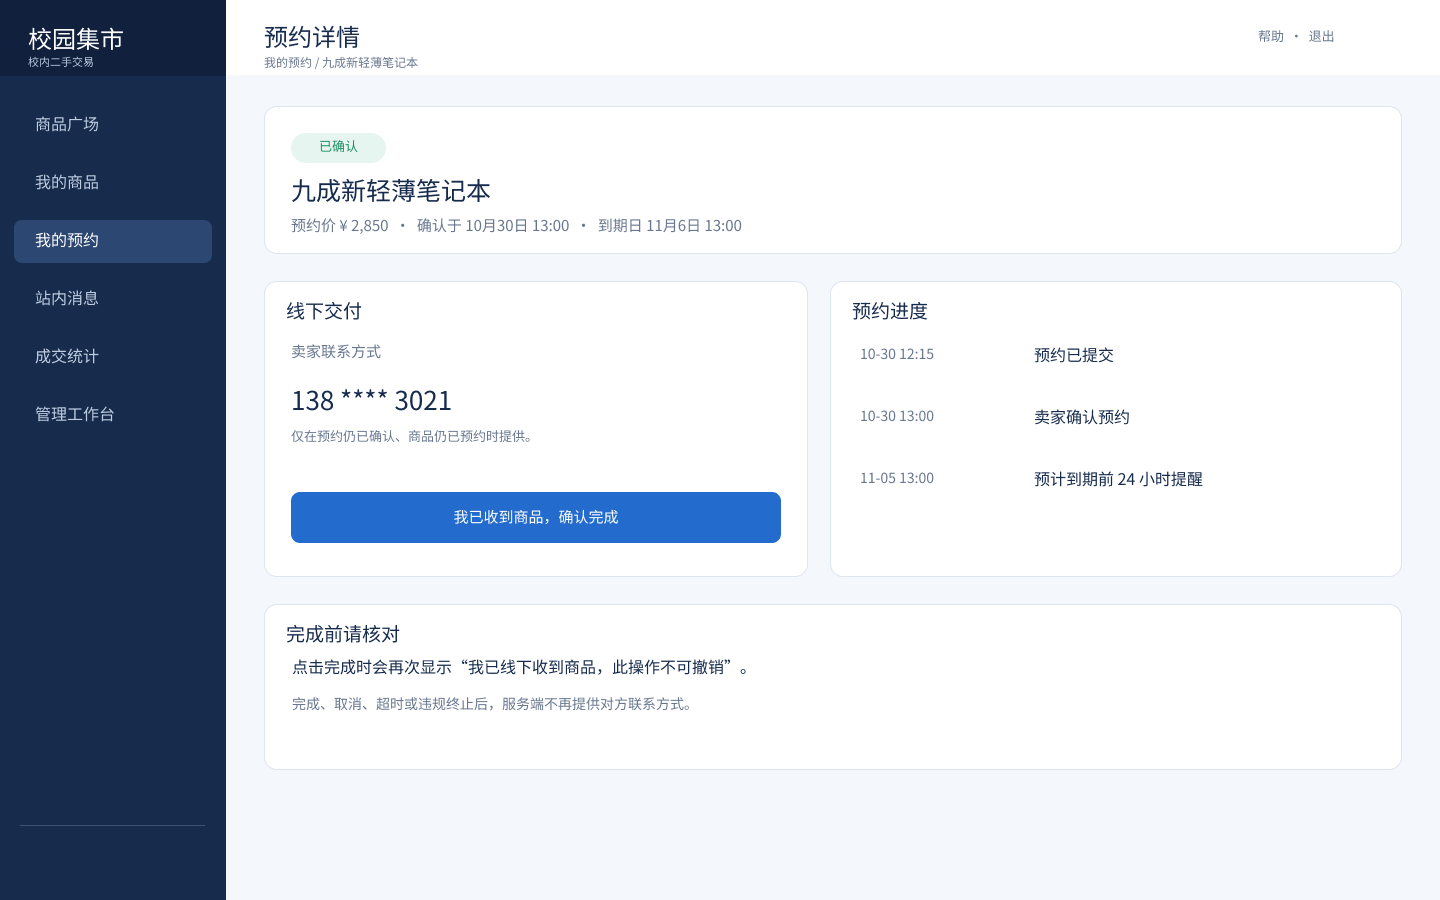
\includegraphics[width=0.88\linewidth,height=\textheight,keepaspectratio,alt={买家预约详情}]{UI界面/06_买家预约详情.png}
\caption{买家预约详情}
\end{figure}

已确认预约可请求对方联系方式，但服务端仍需核对商品``已预约''；终态后刷新即隐藏。完成按钮触发二次确认：``我已线下收到商品，此操作不可撤销''。

\subsubsection{界面 07
站内消息}\label{ux754cux9762-07-ux7ad9ux5185ux6d88ux606f}

\begin{figure}
\centering
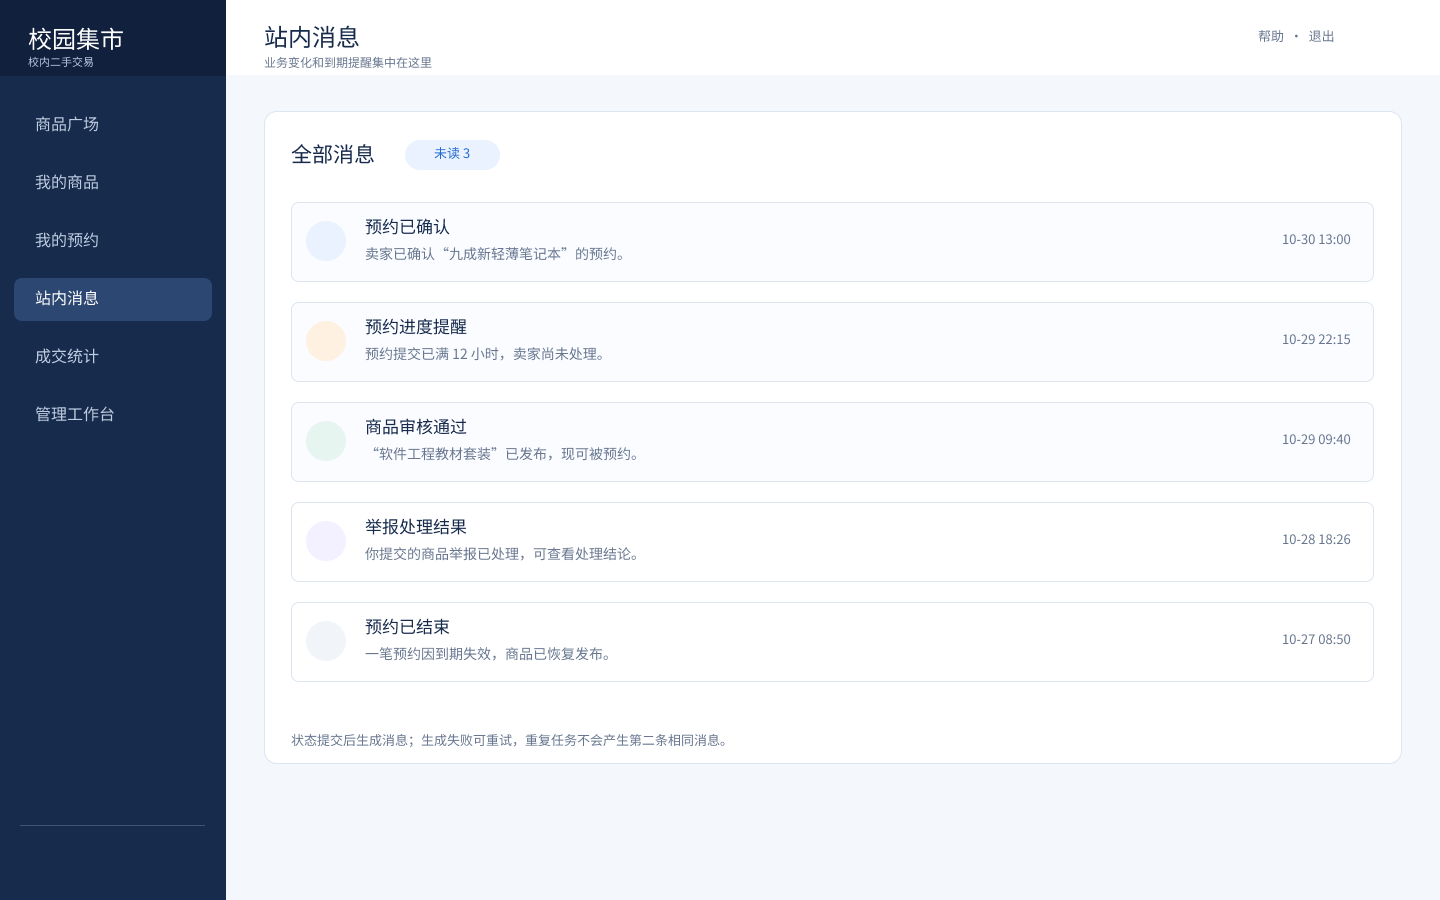
\includegraphics[width=0.88\linewidth,height=\textheight,keepaspectratio,alt={站内消息}]{UI界面/07_站内消息.png}
\caption{站内消息}
\end{figure}

消息列表集中展示审核、预约、举报及到期提醒。待确认满 12
小时仍未处理时给卖家提醒、给买家进度消息；已确认到期前 24
小时且仍有效时提醒双方。

\subsubsection{界面 08
提交举报}\label{ux754cux9762-08-ux63d0ux4ea4ux4e3eux62a5}

\begin{figure}
\centering
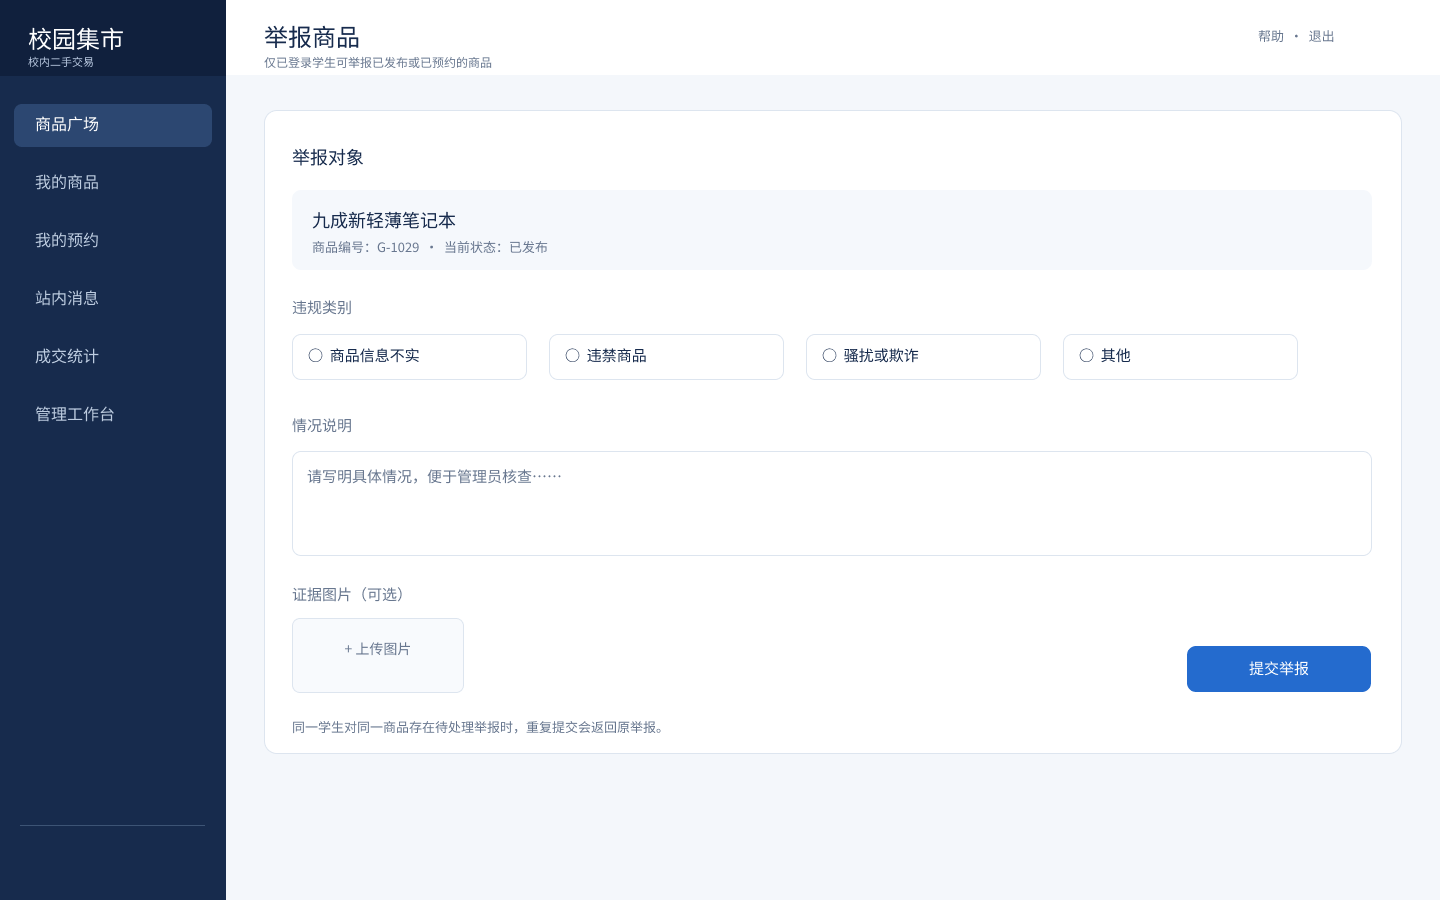
\includegraphics[width=0.88\linewidth,height=\textheight,keepaspectratio,alt={提交举报}]{UI界面/08_提交举报.png}
\caption{提交举报}
\end{figure}

学生选择违规类别、填写说明并可上传证据图片。商品必须仍为已发布或已预约；同一人对同一商品已有待处理举报时，返回原举报。

\subsection{3.2
管理员端界面}\label{ux7ba1ux7406ux5458ux7aefux754cux9762}

\subsubsection{界面 09
商品审核}\label{ux754cux9762-09-ux5546ux54c1ux5ba1ux6838}

\begin{figure}
\centering
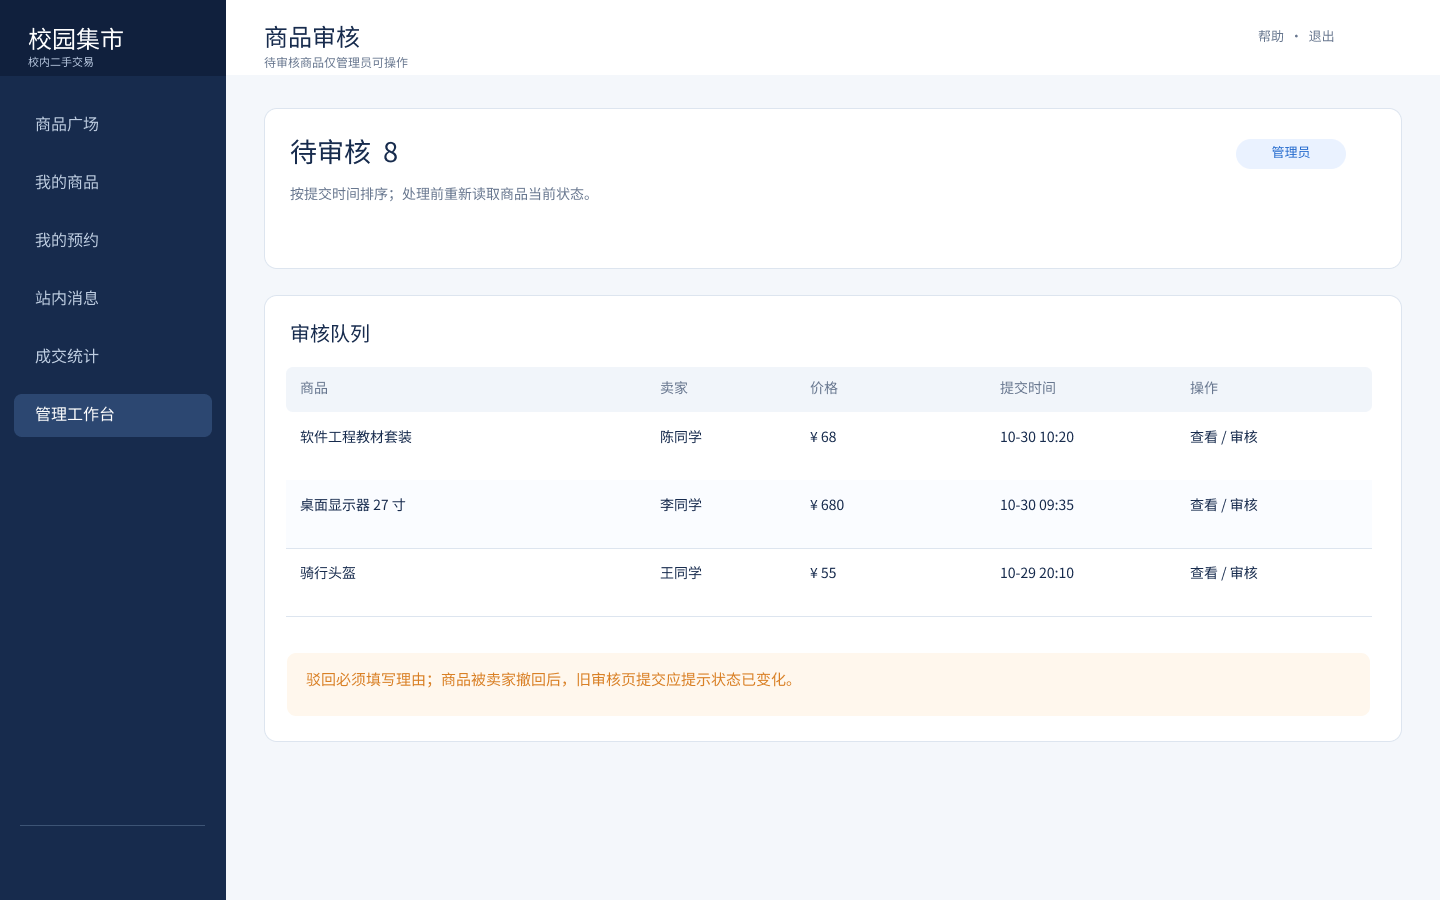
\includegraphics[width=0.88\linewidth,height=\textheight,keepaspectratio,alt={管理员商品审核}]{UI界面/09_管理员商品审核.png}
\caption{管理员商品审核}
\end{figure}

管理员按提交时间处理待审商品。通过发布，驳回必须写理由；若商品已被撤回，旧页面上的审核操作被拒绝。

\subsubsection{界面 10
举报处理}\label{ux754cux9762-10-ux4e3eux62a5ux5904ux7406}

\begin{figure}
\centering
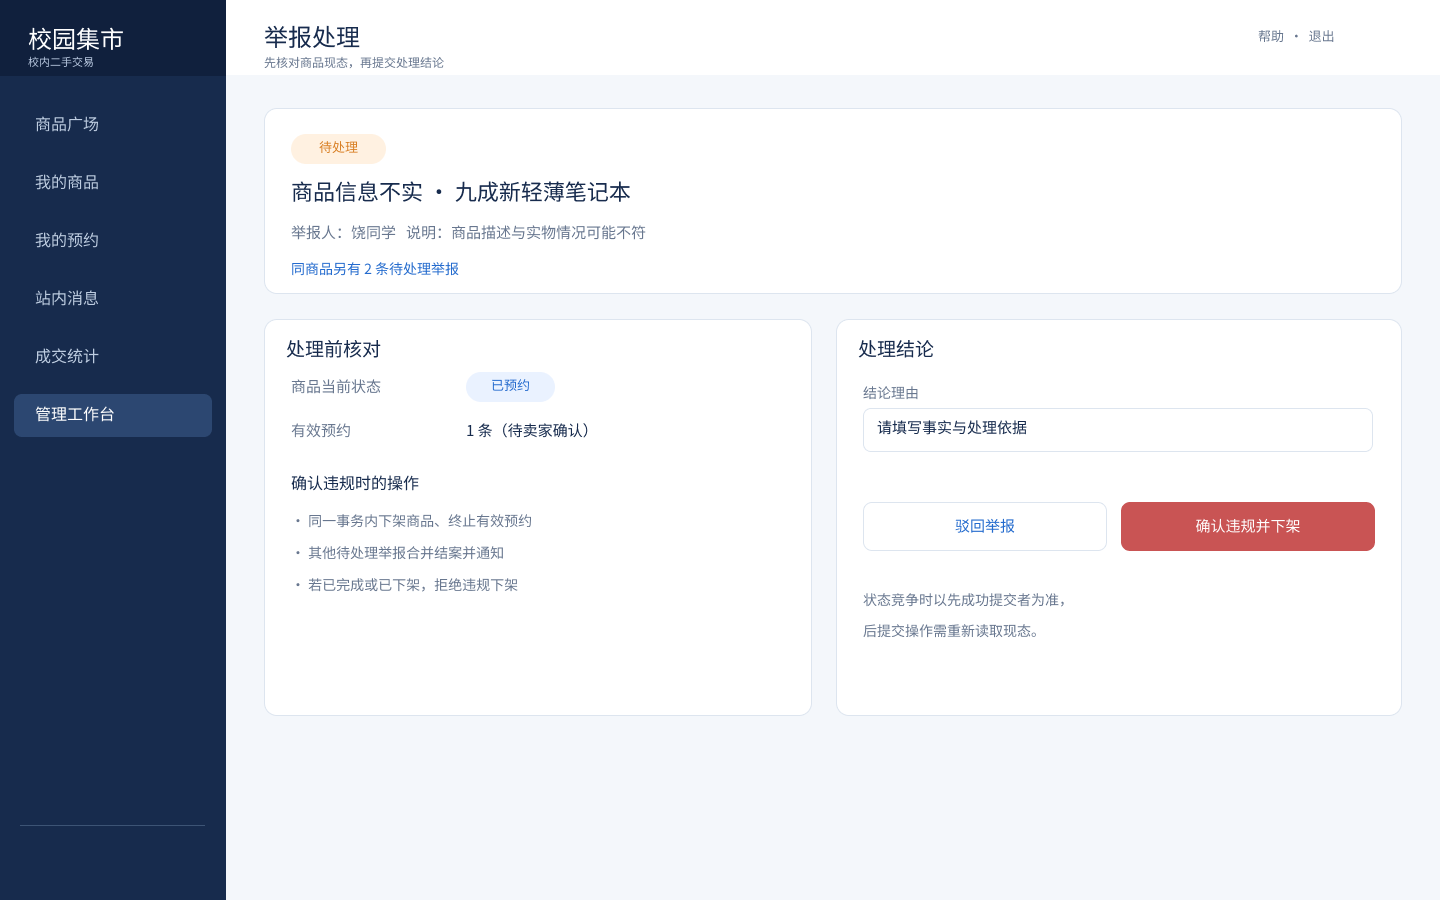
\includegraphics[width=0.88\linewidth,height=\textheight,keepaspectratio,alt={管理员举报处理}]{UI界面/10_管理员举报处理.png}
\caption{管理员举报处理}
\end{figure}

处理页同时显示商品当前状态、有效预约和同商品其他举报。确认违规时事务内下架、终止预约、合并其他待处理举报；若商品已完成或已下架，拒绝该操作并重新读取现态。

\subsubsection{界面 11
统计与日志}\label{ux754cux9762-11-ux7edfux8ba1ux4e0eux65e5ux5fd7}

\begin{figure}
\centering
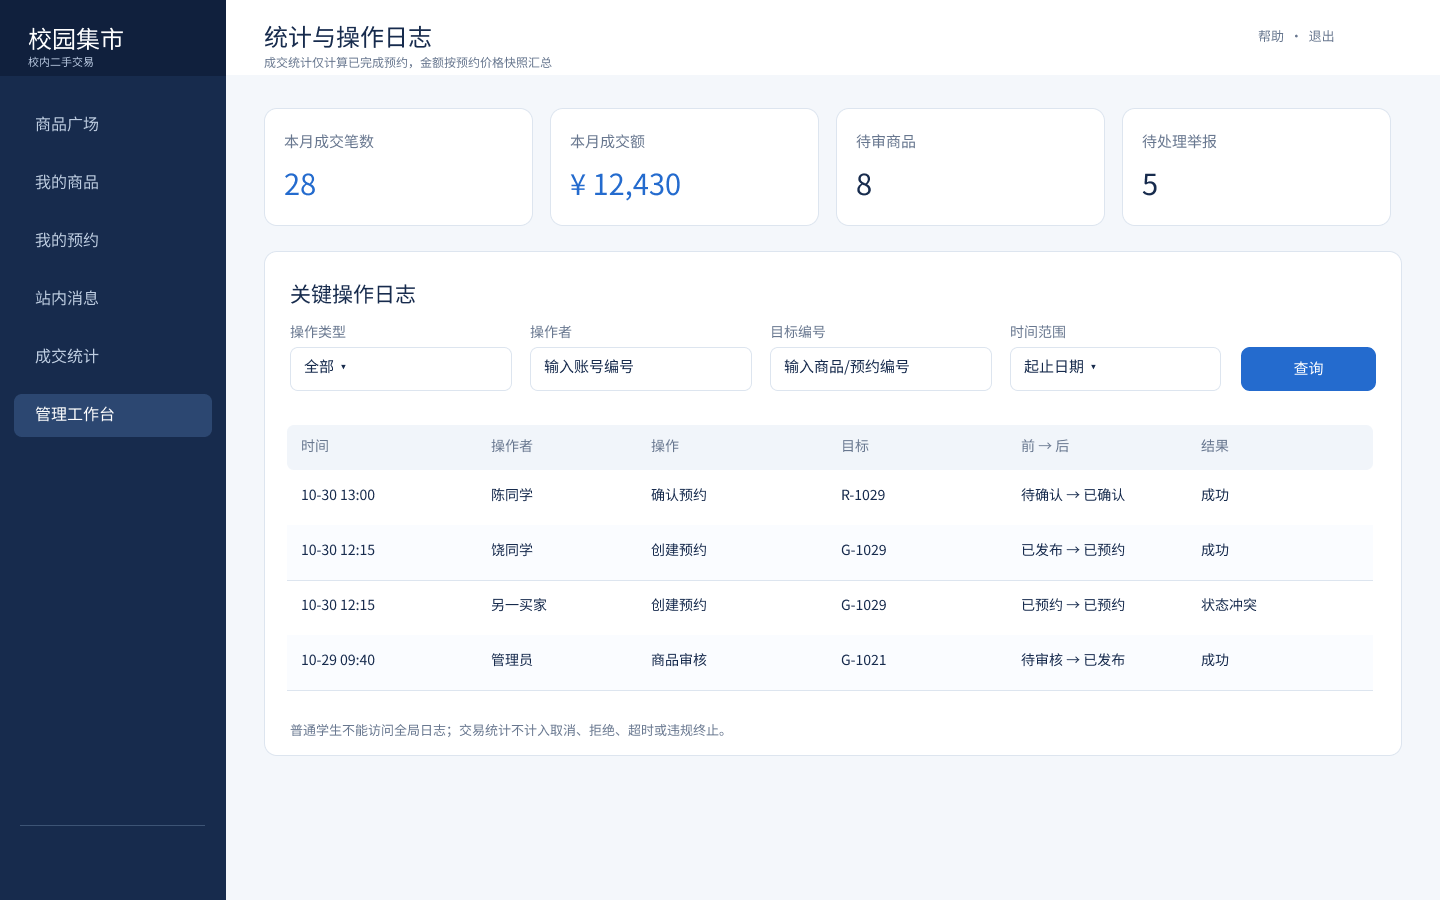
\includegraphics[width=0.88\linewidth,height=\textheight,keepaspectratio,alt={统计与日志}]{UI界面/11_统计与日志.png}
\caption{统计与日志}
\end{figure}

月度成交统计按已完成预约的完成时间和价格快照计算。日志支持按时间、操作者、操作类型、目标编号筛选；普通学生不能进入全局日志页。

\section{4 AI
辅助过程与反思}\label{ai-ux8f85ux52a9ux8fc7ux7a0bux4e0eux53cdux601d}

这次实验把 Codex 用在需求整理、UML
绘制、界面草拟和报告修改上。使用前先从实验一的需求中挑出并发预约、重复提交、举报处理和联系方式访问这几条容易出错的规则，再让工具给出图和界面的候选方案。下面按实际使用顺序记录生成结果、发现的问题和修改过程。

\subsection{4.1 使用记录}\label{ux4f7fux7528ux8bb0ux5f55}

{\def\LTcaptype{none} % do not increment counter
\begin{longtable}[]{@{}
  >{\raggedright\arraybackslash}p{(\linewidth - 6\tabcolsep) * \real{0.2500}}
  >{\raggedright\arraybackslash}p{(\linewidth - 6\tabcolsep) * \real{0.2500}}
  >{\raggedright\arraybackslash}p{(\linewidth - 6\tabcolsep) * \real{0.2500}}
  >{\raggedright\arraybackslash}p{(\linewidth - 6\tabcolsep) * \real{0.2500}}@{}}
\toprule\noalign{}
\begin{minipage}[b]{\linewidth}\raggedright
使用场景
\end{minipage} & \begin{minipage}[b]{\linewidth}\raggedright
AI 生成结果
\end{minipage} & \begin{minipage}[b]{\linewidth}\raggedright
检查时发现的问题
\end{minipage} & \begin{minipage}[b]{\linewidth}\raggedright
调整后的结果
\end{minipage} \\
\midrule\noalign{}
\endhead
\bottomrule\noalign{}
\endlastfoot
梳理架构 & Codex 根据实验要求和 REQ-001---REQ-027
整理出六个业务模块和组件图初稿。 &
模块列得比较全，但初稿容易让人以为每个模块都是独立服务，也没有充分强调跨模块事务。
&
第一版改为单体后端中的逻辑模块；商品、预约和举报的相关状态变更共用事务，通知在业务提交后处理。 \\
绘制 UML & 生成类图、组件图、用例图、商品与预约状态图、预约时序图共六份
PlantUML 源码。 &
图能通过语法检查不等于业务正确。类图初稿只把请求回执连到学生，漏掉了管理员操作。
& 在类图中引入 Account 父类，让 Student、Admin 都关联
RequestReceipt，并补充审核字段和预约请求编号。 \\
草拟 UI &
按功能清单生成十一张桌面端界面草稿，统一了导航、卡片和状态标签。 &
草稿用 ReportLab 绘制；转换成 SVG
后文字成为路径，不便在设计工具里继续改。预约页的未来提醒也容易被看成已经发生的消息。
& 把提醒文案改成``预计到期前 24 小时提醒''，并决定在 Figma
中重建正式界面。 \\
修改报告与核对图片 & 生成模块说明、图的设计理由、界面说明和 AI
使用记录的初稿，并整理 LaTeX 排版。 &
有些句子像工具在评价实验，也会把设计方案写得像已实现功能；初版 UML
位图中的中文标题缩放后不够清晰。 &
调整为完成实验时的自然叙述，区分``设计原型''\,``拟采用''和``已经完成''的工作；核对标题文字并重新导出高清
UML 图，再检查 PDF 中的排版。 \\
\end{longtable}
}

\subsection{4.2
设计取舍与工具局限}\label{ux8bbeux8ba1ux53d6ux820dux4e0eux5de5ux5177ux5c40ux9650}

设计时采用``先列规则、后画图''的顺序。实验一中最容易出错的是并发预约、重复请求、举报状态竞争和联系方式访问条件，因此选了预约时序图与两个状态图，而没有为了凑数量画与业务关系不大的对象图。UI
则先列出功能模块清单，再检查每页是否有相应的操作入口和状态提示。Figma
重做也暴露了草稿的局限：图片看起来完整，不代表文字和控件便于后续修改。

大模型适合把长需求拆为模块、提出类和交互的候选结构、生成便于反复修改的
PlantUML
代码，也能较快制作统一风格的界面草图。它的局限是可能补出看似合理、但未经确认的规则；图能渲染也不代表业务正确。比如数据库约束容易被一句``只允许一个预约''带过，异步消息也可能被误画进交易事务，界面还可能提前暴露联系方式。处理这些问题时，逐条回看
REQ 编号，检查终态和竞态，并把待确认参数留空。

从这次体验看，较合适的工作流是``需求编号 → AI 生成候选图和界面 →
检查文件、语法与渲染 → 核对业务规则和可编辑性 →
修改并记录版本''。这样可以把更多时间放在检查和决策上，但检查不能只停留在错别字：状态是否允许转换、并发时谁生效、信息何时可见，仍需结合原始需求作判断。Figma
导出图替换 ReportLab
草稿，就是本次发现工具产物不适合最终交付后作出的一次调整。


\end{document}
